\begin{frame}
    \frametitle{Universal Approximation Theorem for operators}
    \footnotesize
    Let,
    \begin{itemize}
        \item \(\sigma\) - a continuous non-polynomial function
        \item \(X\) - Banach space
        \item \(K_1 \in X, \ K_2 \in \mathbb{R}^d\) - two compact sets
        \item \(V \in C(K_1)\) - a compact set in functional space of \(K_1\)
        \item \(G\) - non-linear continuous operator that maps \(V \to C(K_2)\)
    \end{itemize}

    Then for any \(\epsilon > 0 \), there are positive integers \(n,p,m\),
    constants \(c_i^k,\varepsilon_{ij}^k,\theta_i^k,\zeta_k \in \mathbb{R}, \ w_k \in \mathbb{R}^d, \ x_j \in K_1, \ i = 1,..,n, \ k = 1,...,p, \)
    \( j = 1,...,m \) such that


    \begin{align}
        \left| G(u)(y) - \sum_{k=1}^{p}\underbrace{\sum_{i=1}^{n} c_i^k \sigma\left(\sum_{j=1}^m \varepsilon_{ij}^k u(x_j) + \theta_i^k\right)}_\text{branch}\underbrace{\sigma\left(w_k.y + \zeta_k\right)}_\text{trunk} \right| < \epsilon
    \end{align}

    holds for \(u \in V\) and \(y \in K_2\).
\end{frame}

%------------------------------------------------------------------------------
\begin{frame}
    \frametitle{Univeral Approx. Thm for operators }
    In other form, \footcite{goswami2023physics}

    \begin{align}
        \left| G(u)(y) - \sum_{k=1}^p \underbrace{br_k\left(u(x_1),u(x_2),...,u(x_m)\right)}_\text{branch} \underbrace{tr_k\left(y\right)}_\text{trunk} \right| < \epsilon
    \end{align}


    where, \(x_1,...,x_m\) are called sensor points.\\

    \vspace{1.0cm}
    The functions \(br(), \ tr()\), can be approximated by neural networks \footcite{hornik1989multilayer}

\end{frame}

%------------------------------------------------------------------------------
\begin{frame}
    \frametitle{Data-driven deep-o-net example}

    The operator \(G: sin(\omega t) \to \omega cos(\omega t)\)
    \begin{figure}
       \center
        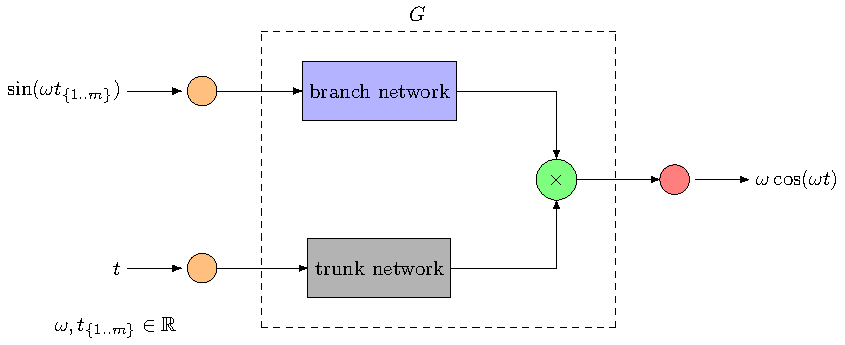
\includegraphics[scale=0.8]{supportingFiles/schematics/01_sineExample/Don_example.pdf}
    \end{figure}
\end{frame}

\begin{frame}
    \frametitle{Data-driven deep-o-net example - results}
    \hbox{\hspace{-1cm}
        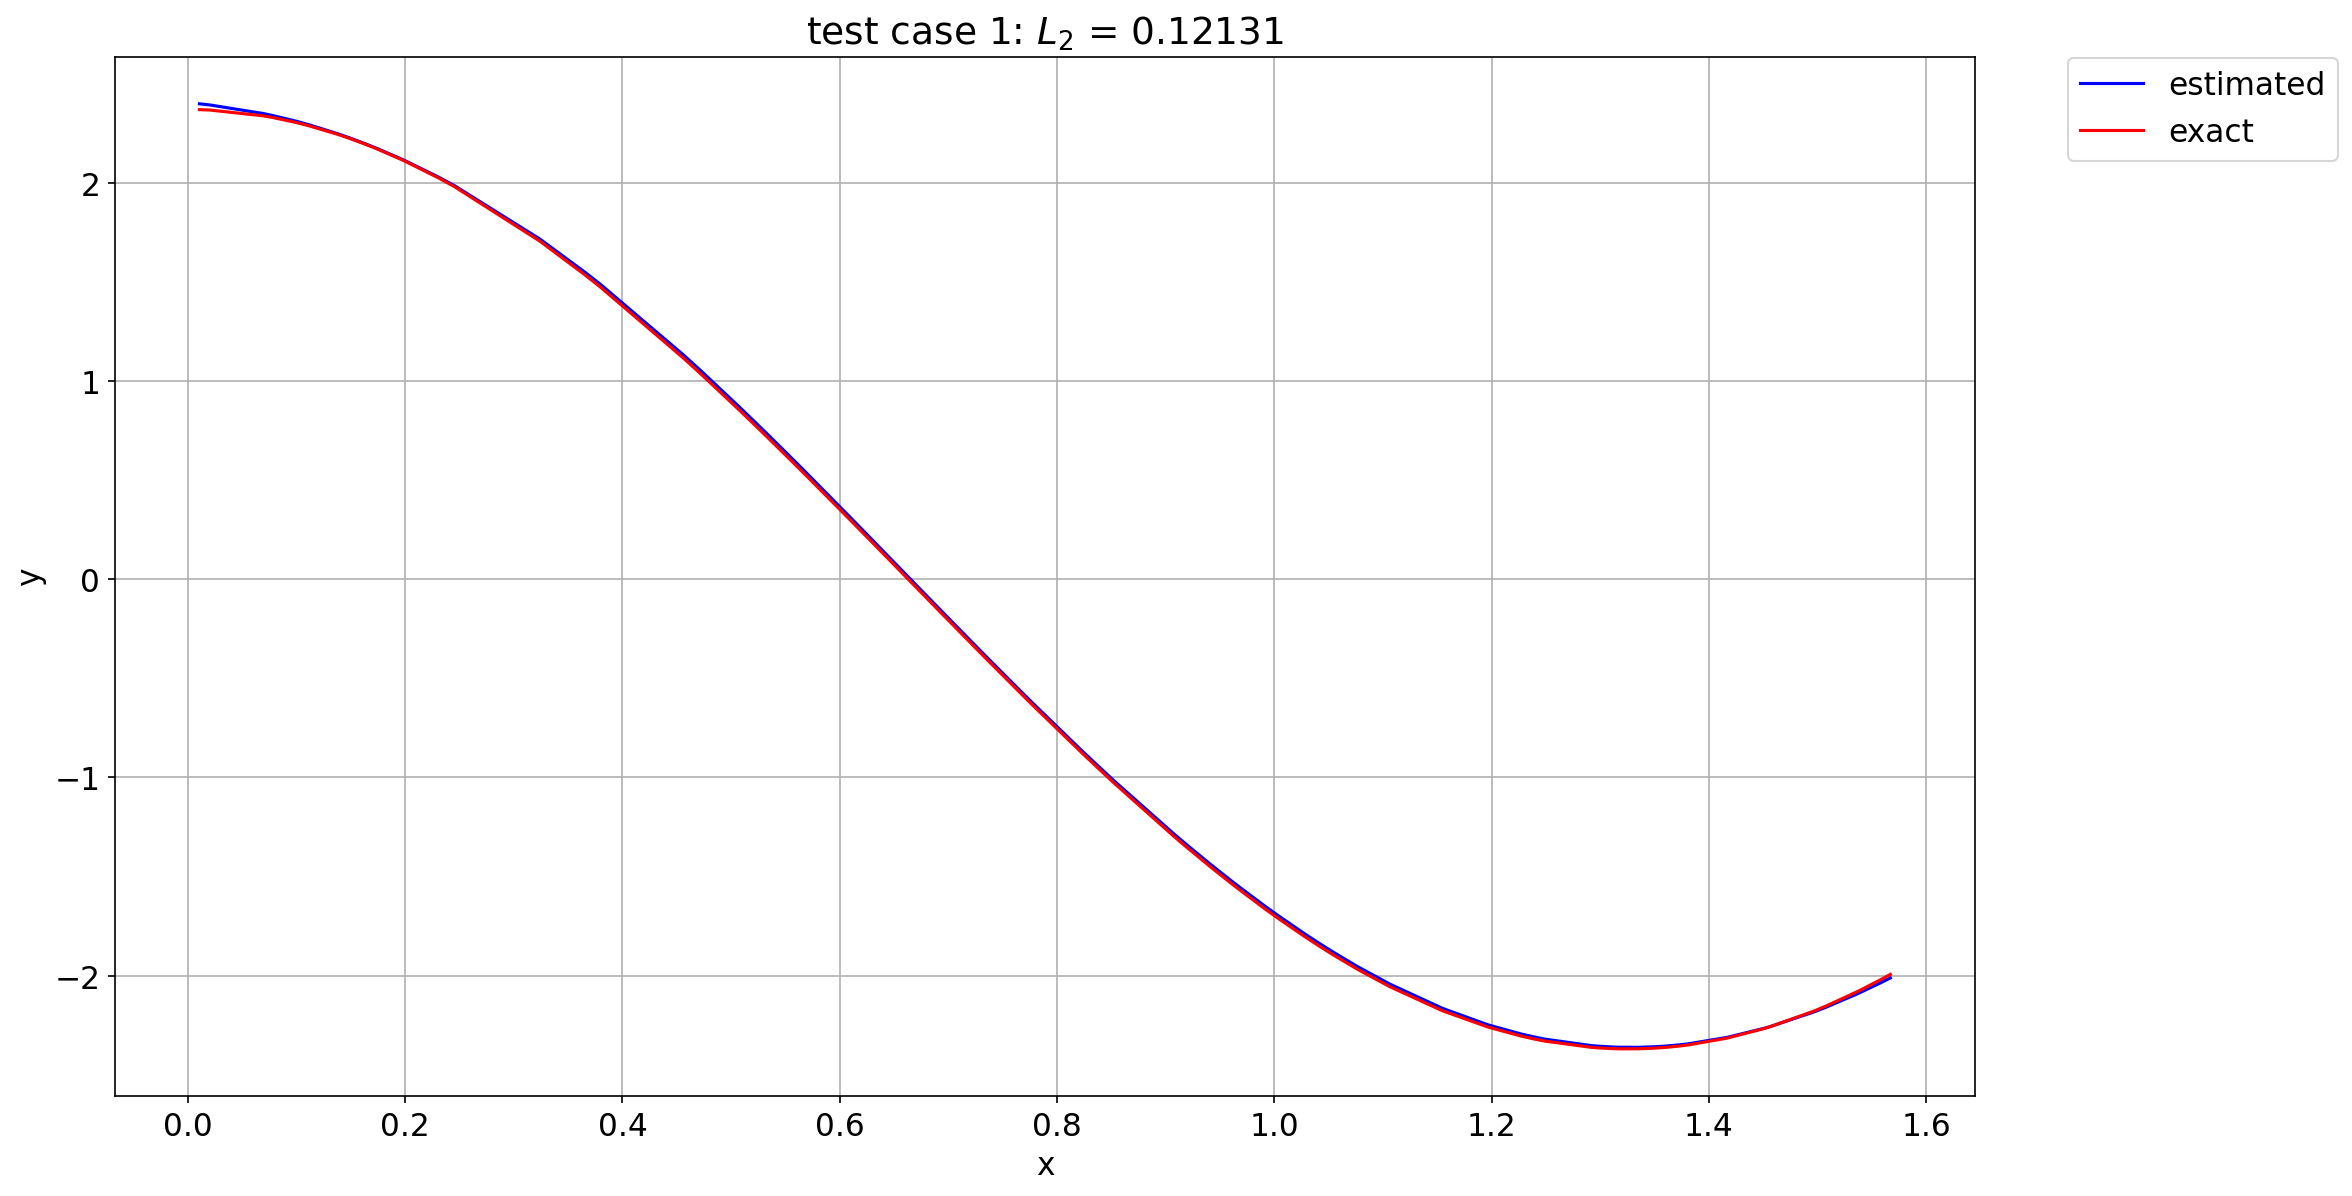
\includegraphics[scale=0.32]{supportingFiles/DON_results/test_case_1.png}\hspace{5cm}
    }
\end{frame}

\begin{frame}
    \frametitle{Data-driven deep-o-net example - results}
    \hbox{\hspace{-1cm}
        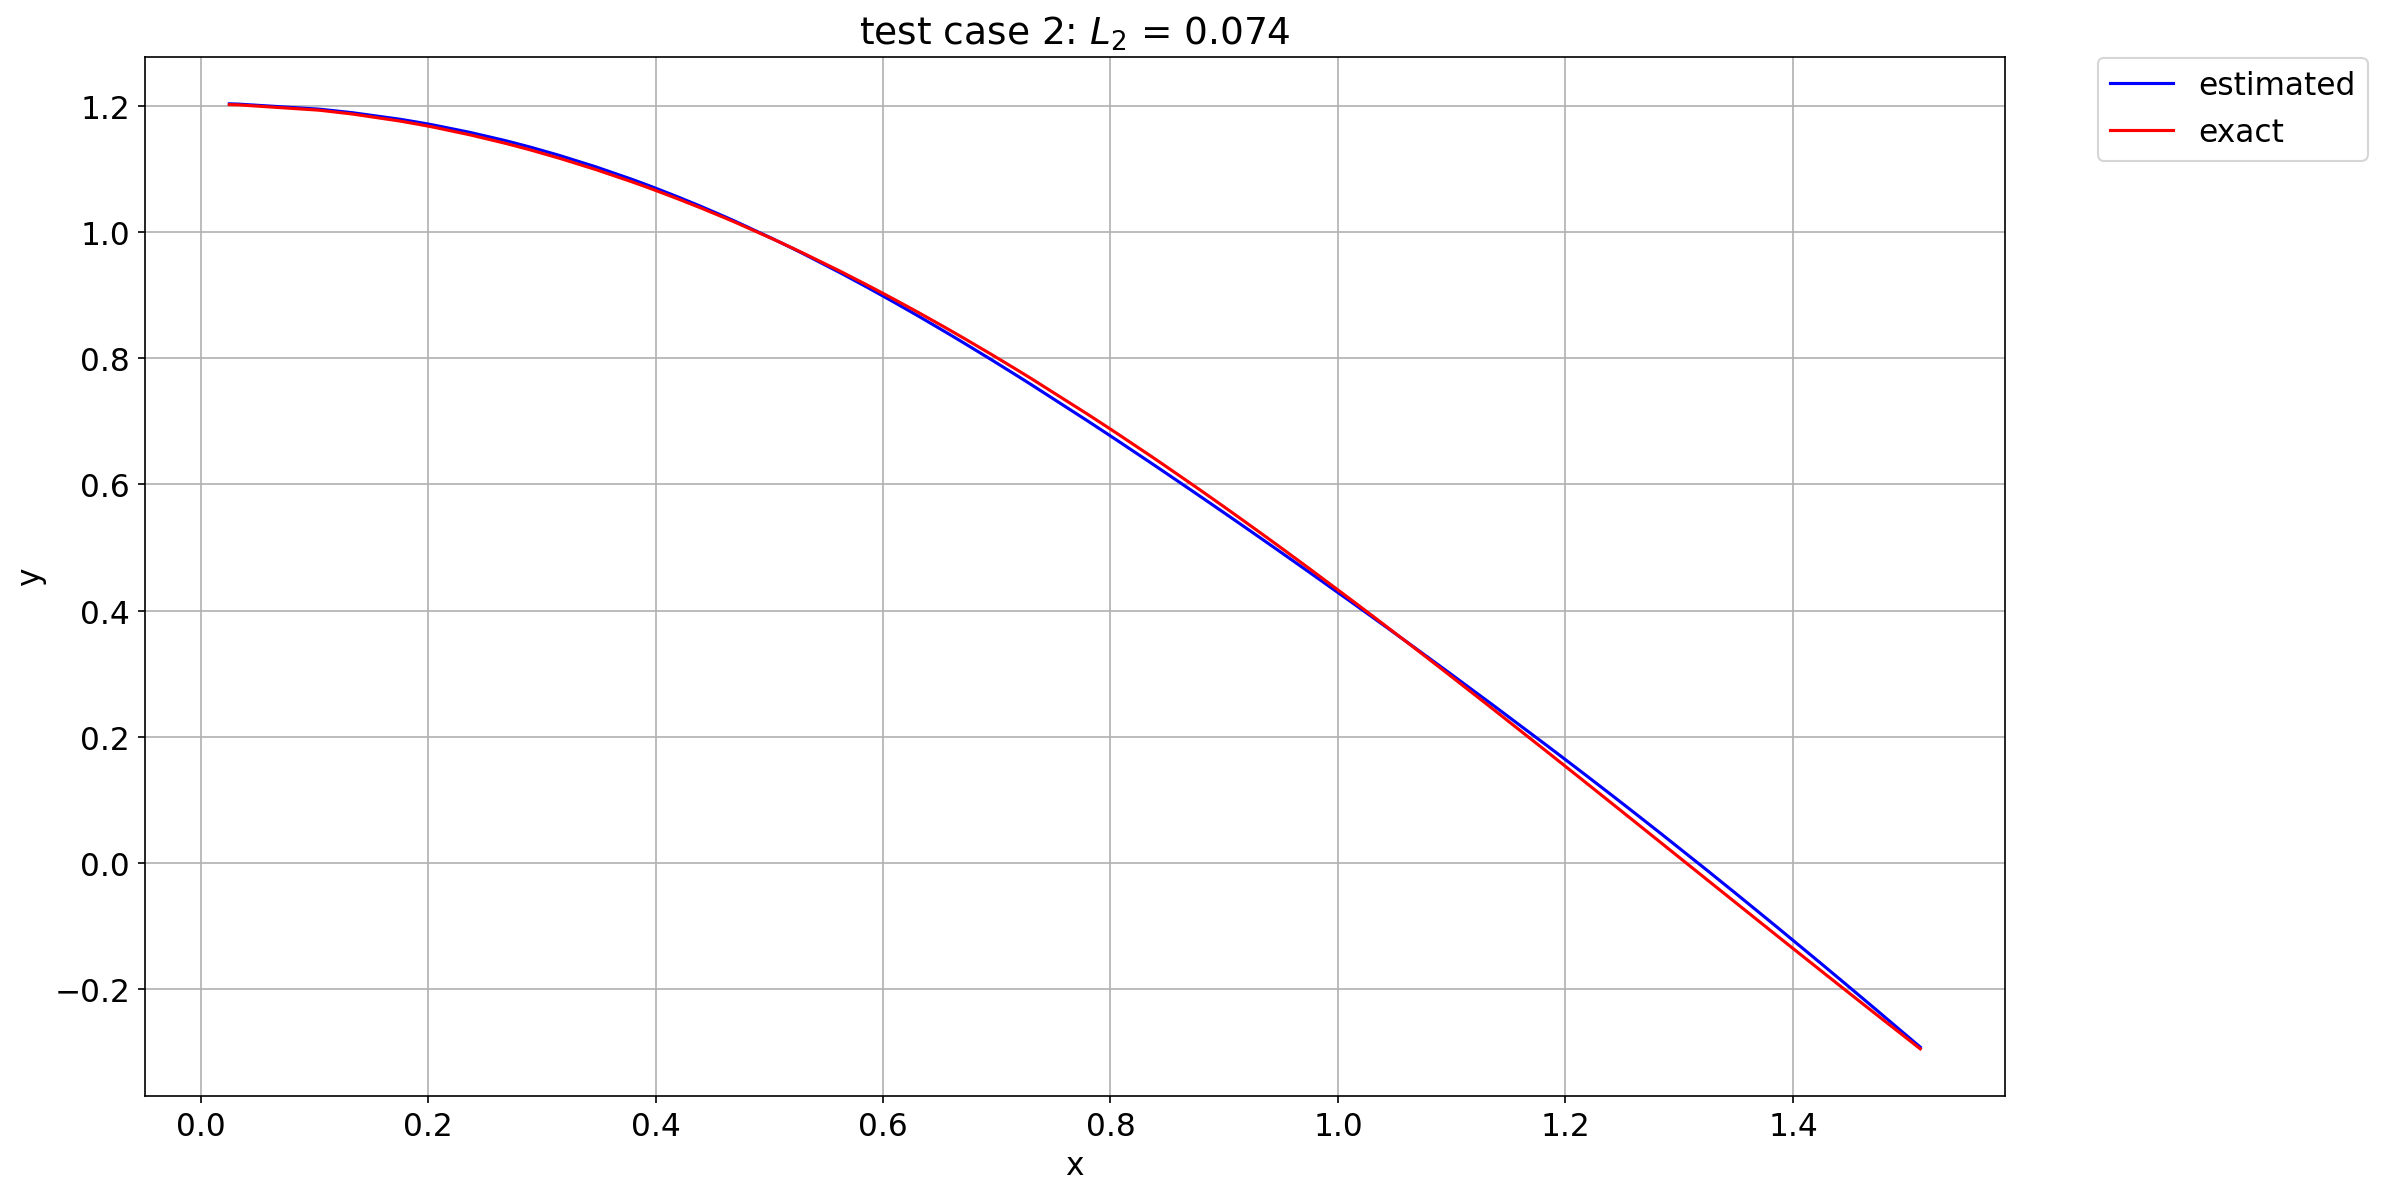
\includegraphics[scale=0.32]{supportingFiles/DON_results/test_case_2.png}\hspace{5cm}
    }
\end{frame}

\begin{frame}
    \frametitle{Data-driven deep-o-net example - results}
    \hbox{\hspace{-1cm}
        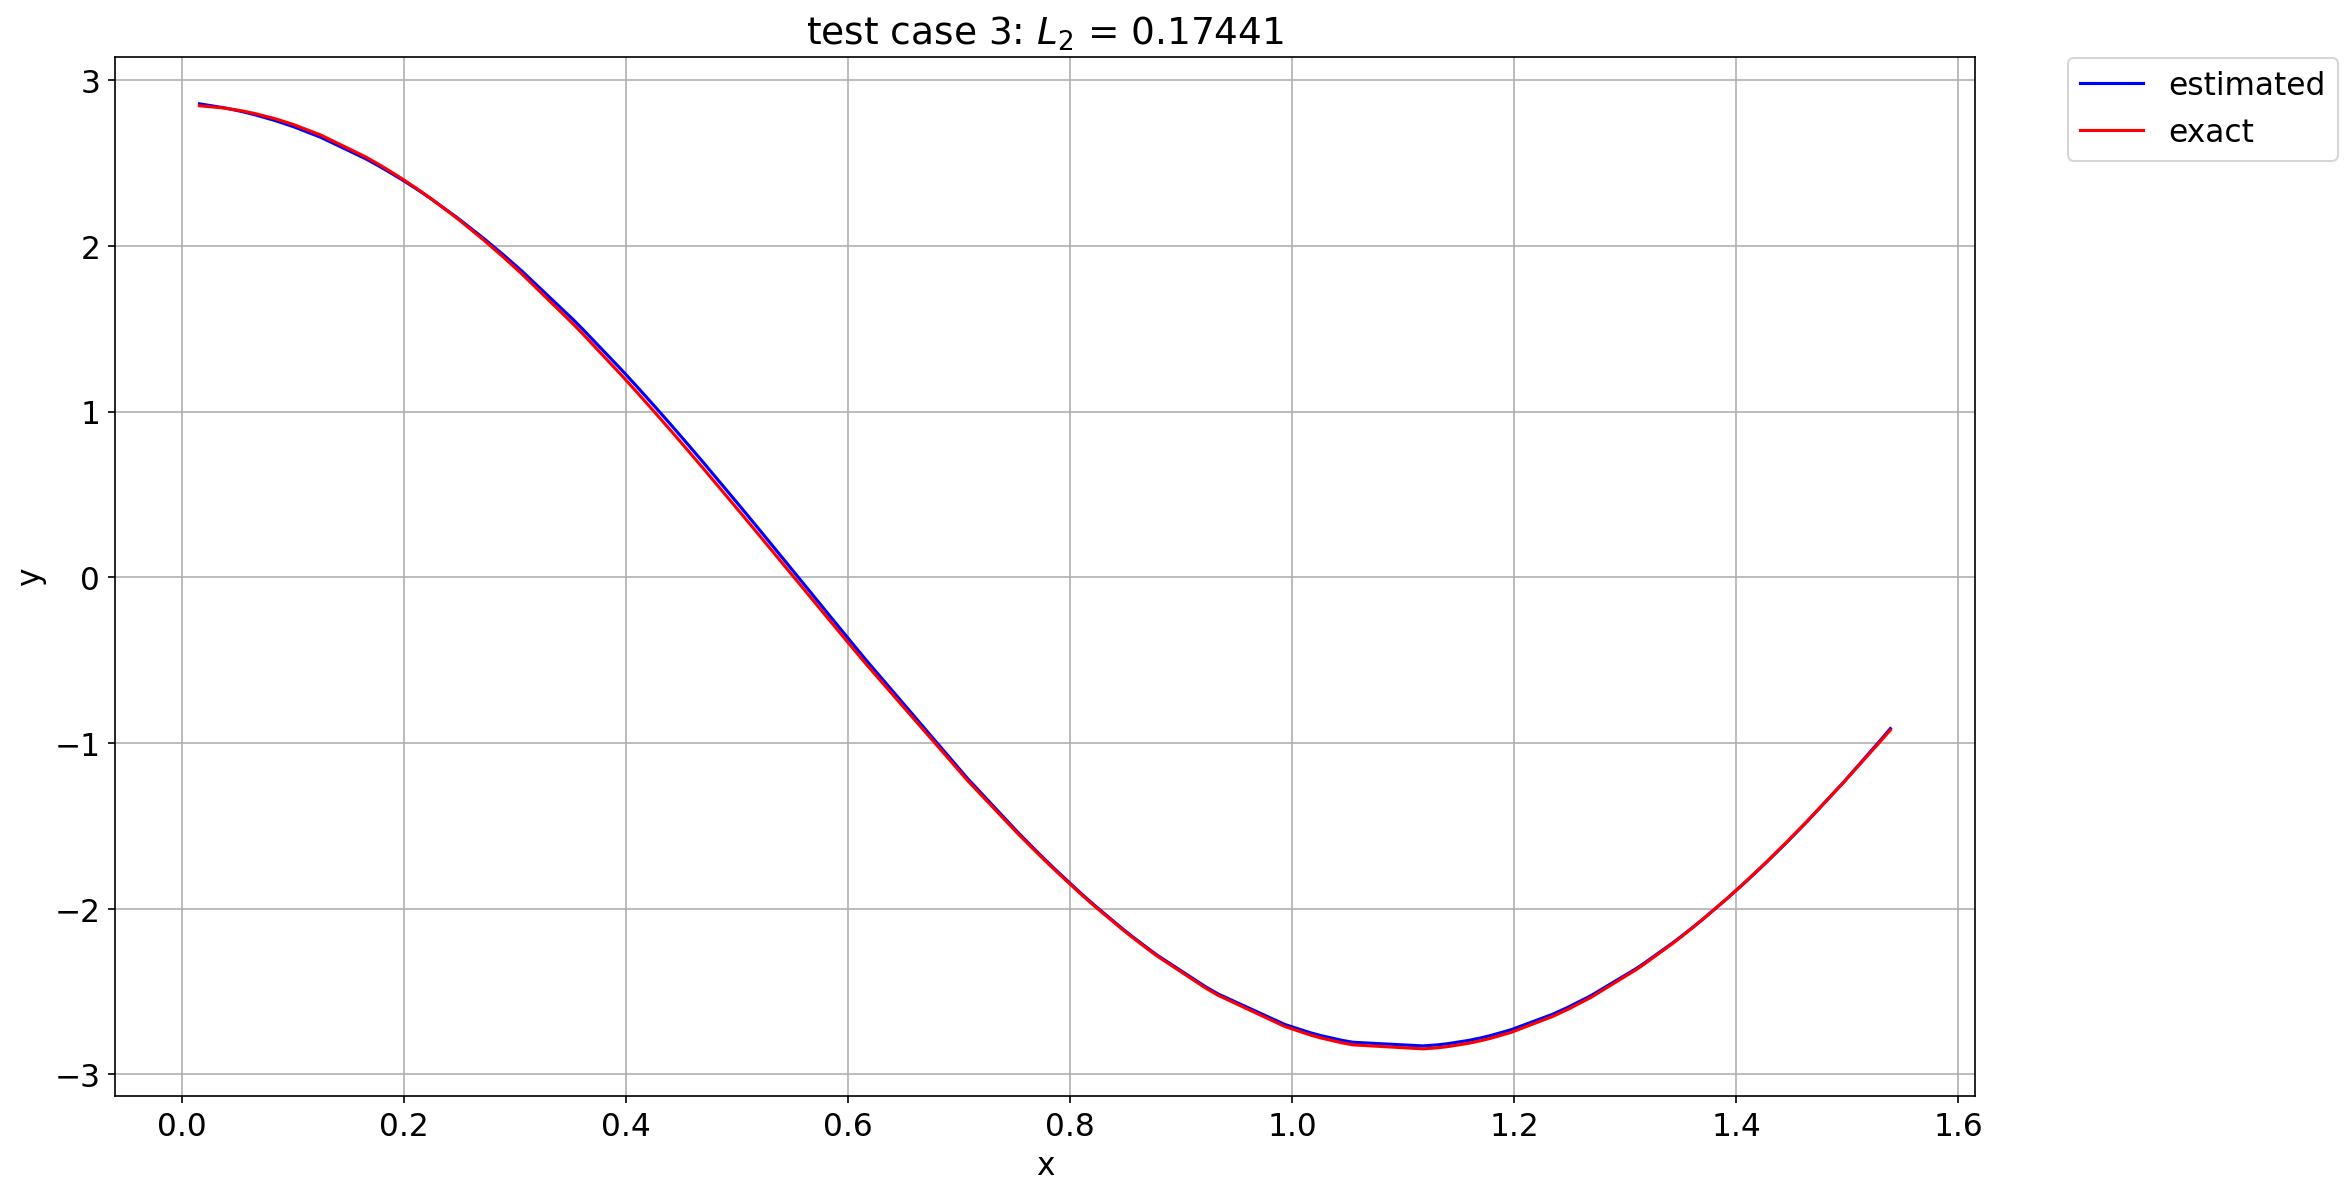
\includegraphics[scale=0.32]{supportingFiles/DON_results/test_case_3.png}\hspace{5cm}
    }
\end{frame}

\begin{frame}
    \frametitle{Data-driven deep-o-net example - results}
    \hbox{\hspace{-1cm}
        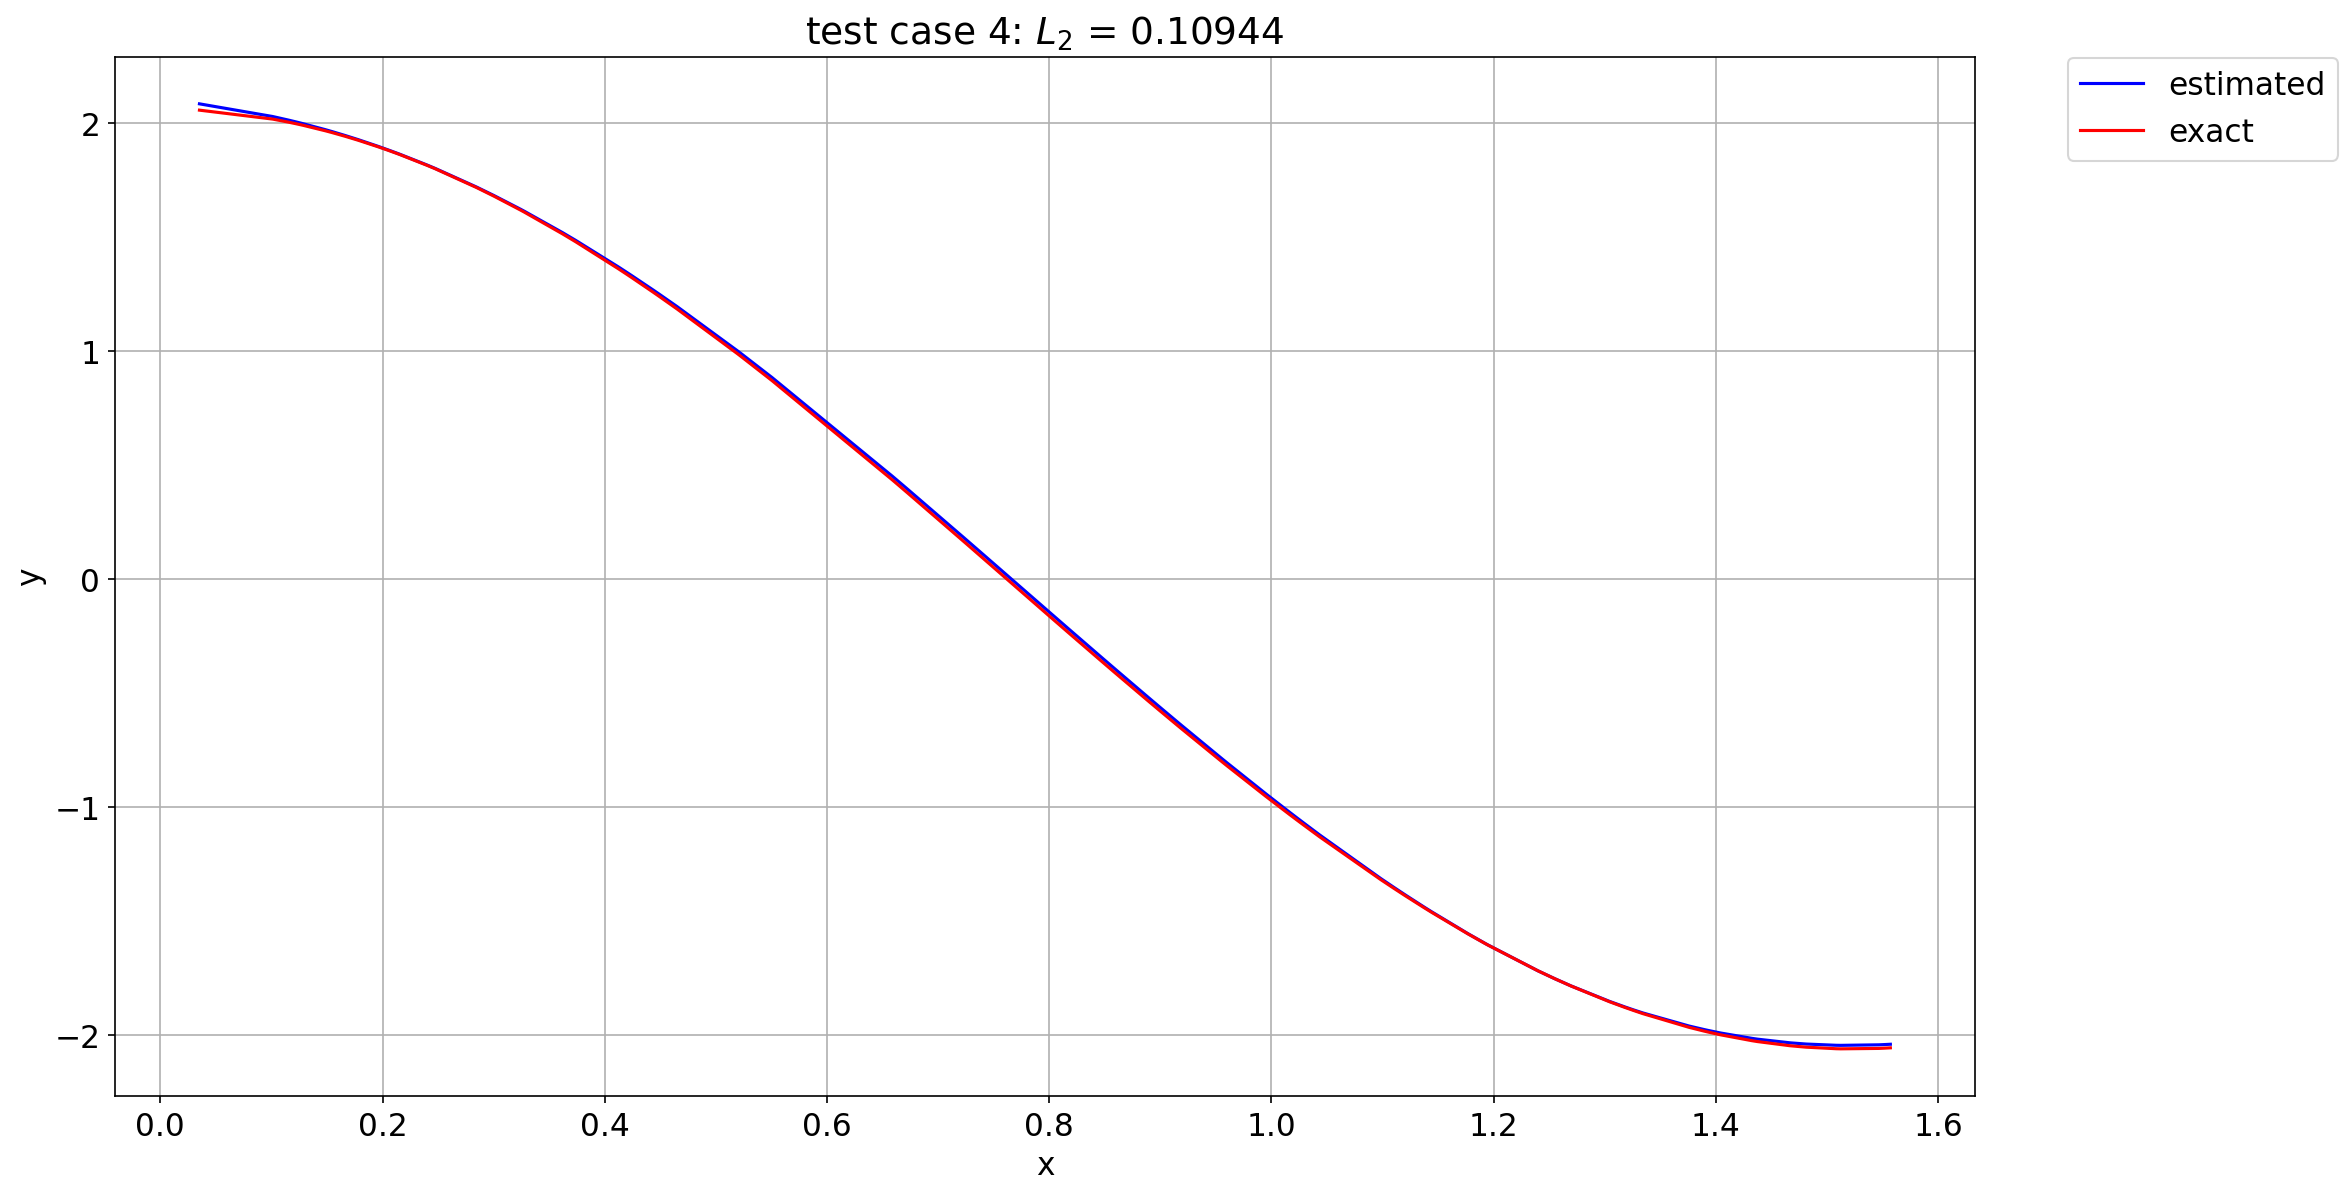
\includegraphics[scale=0.32]{supportingFiles/DON_results/test_case_4.png}\hspace{5cm}
    }
\end{frame}

\begin{frame}
    \frametitle{Data-driven deep-o-net example - results}
    \hbox{\hspace{-1cm}
        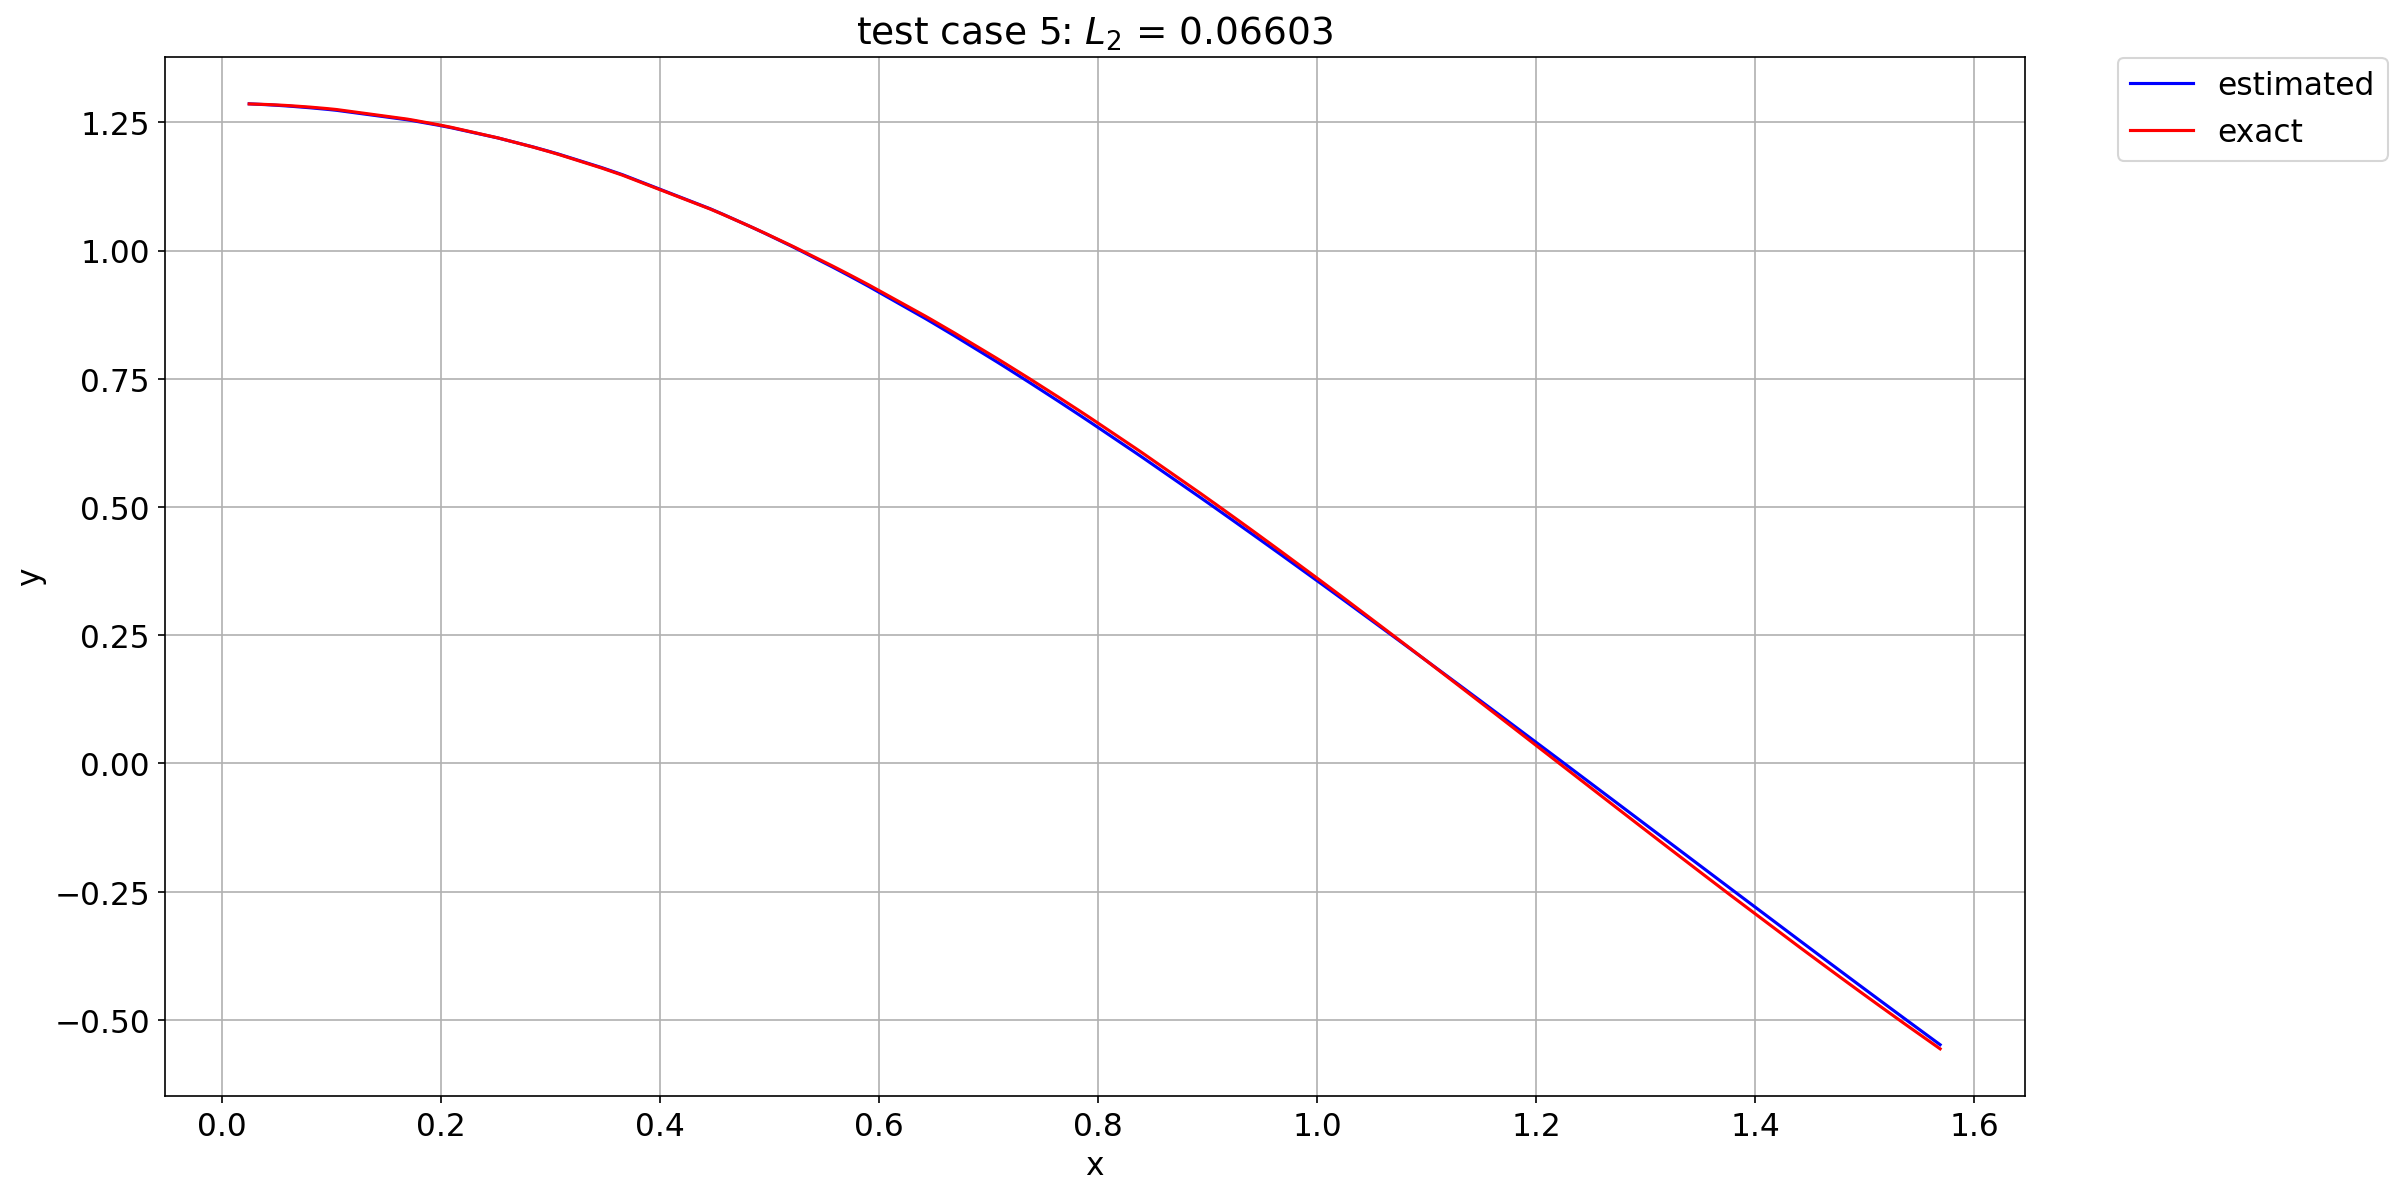
\includegraphics[scale=0.32]{supportingFiles/DON_results/test_case_5.png}\hspace{5cm}
    }
\end{frame}

%------------------------------------------------------------------------------
\begin{frame}
    \frametitle{Data-driven deep-o-net Experiment}
    \onslide<2->{
        Does it really approximate an Operator alone?
    }

    \onslide<3->{
        Mathematically not! \\
    }

    \onslide<4->{
        With a trained model, tried evaluating \\
        \(\hat{G}: \cos(\omega t) \to -\omega\sin(\omega t) \)
    }

    \onslide<5->{
        \begin{figure}
            \center
            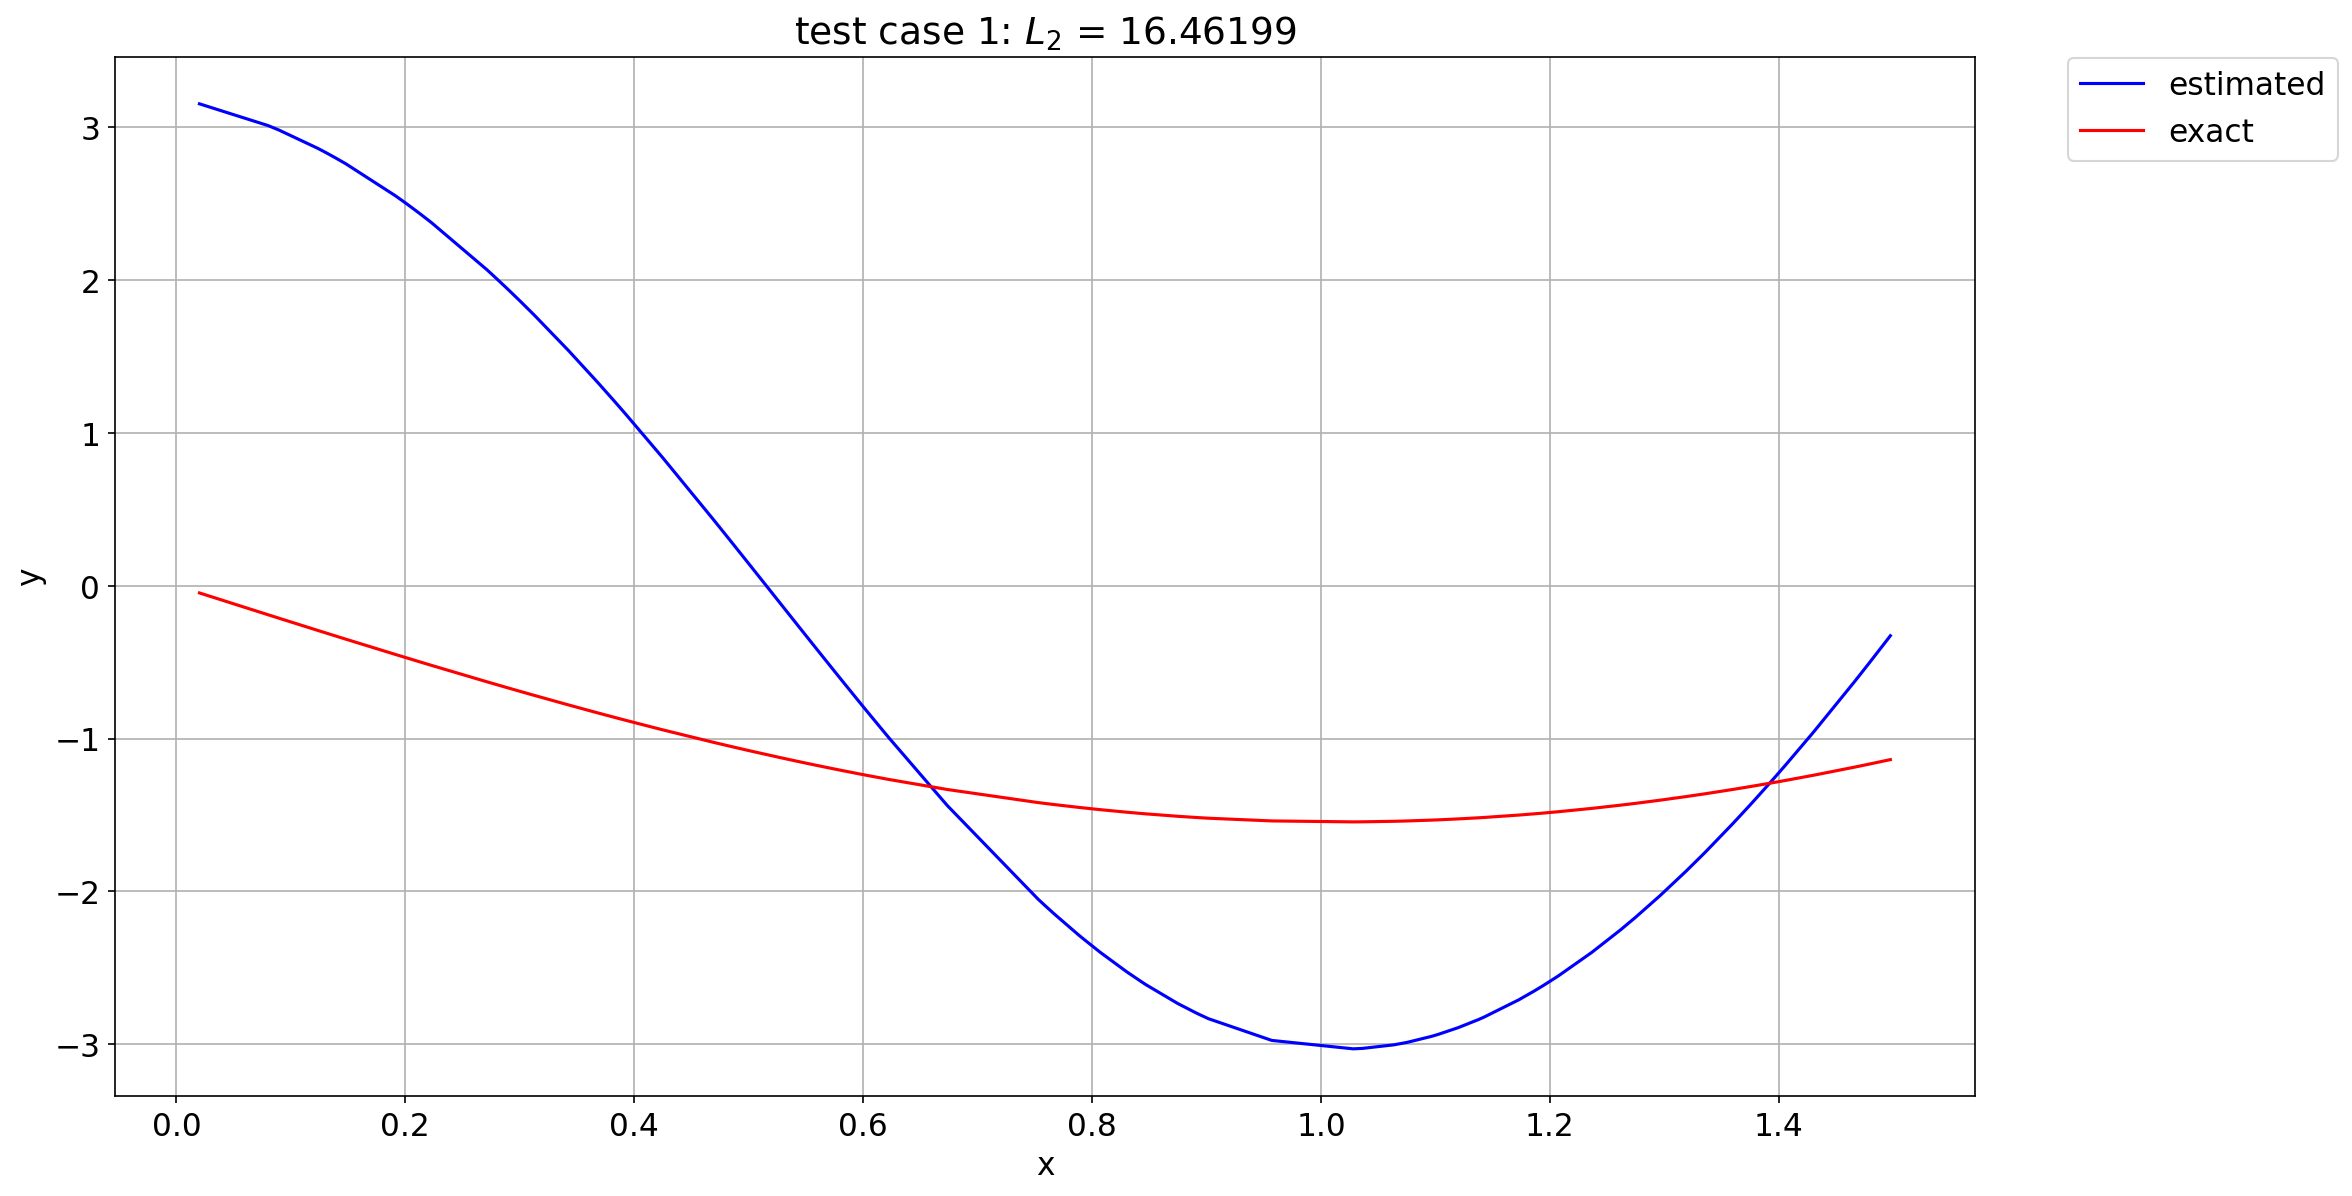
\includegraphics[scale=0.22]{supportingFiles/DON_results/inverseTest/test_case_1.png}
        \end{figure}
    }

    \onslide<6->{
        Network approximates \textcolor{blue} {Operator with encoded input function}
    }

\end{frame}

%------------------------------------------------------------------------------
\begin{frame}
    \frametitle{Physics Informed Deep-o-net}
    \onslide<2->{
        Tried with operator, \(G: \cos(\omega t) \to x\)
    } \\
    \onslide<3->{
        with constraint, \(\dot{x} = \cos(\omega t)\)
    }
    \onslide<4->{
        \begin{figure}
            \center
            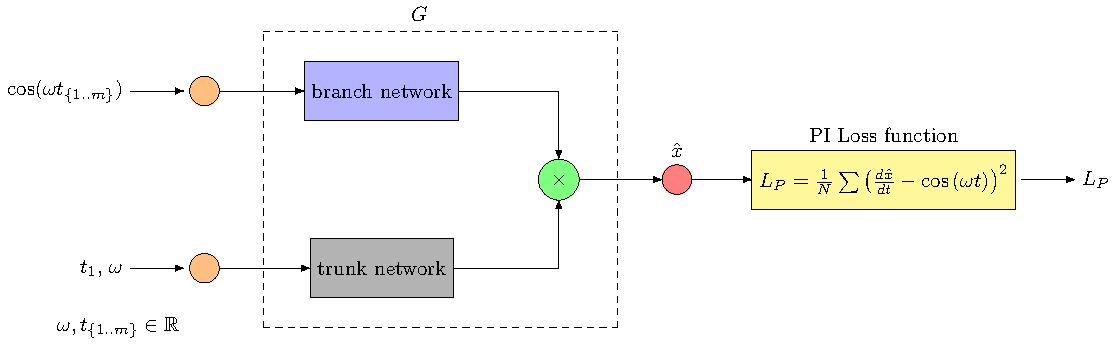
\includegraphics[scale=0.6]{supportingFiles/schematics/02_PI_example/PI_example.pdf}
        \end{figure}
    }
    \vspace{1cm}
    \onslide<5->{
        This includes automatic differentiation, \(\dot{x}\)
    }
\end{frame}

\begin{frame}
    \frametitle{Physics Informed Deep-o-net - results}
    \hbox{\hspace{-1cm}
        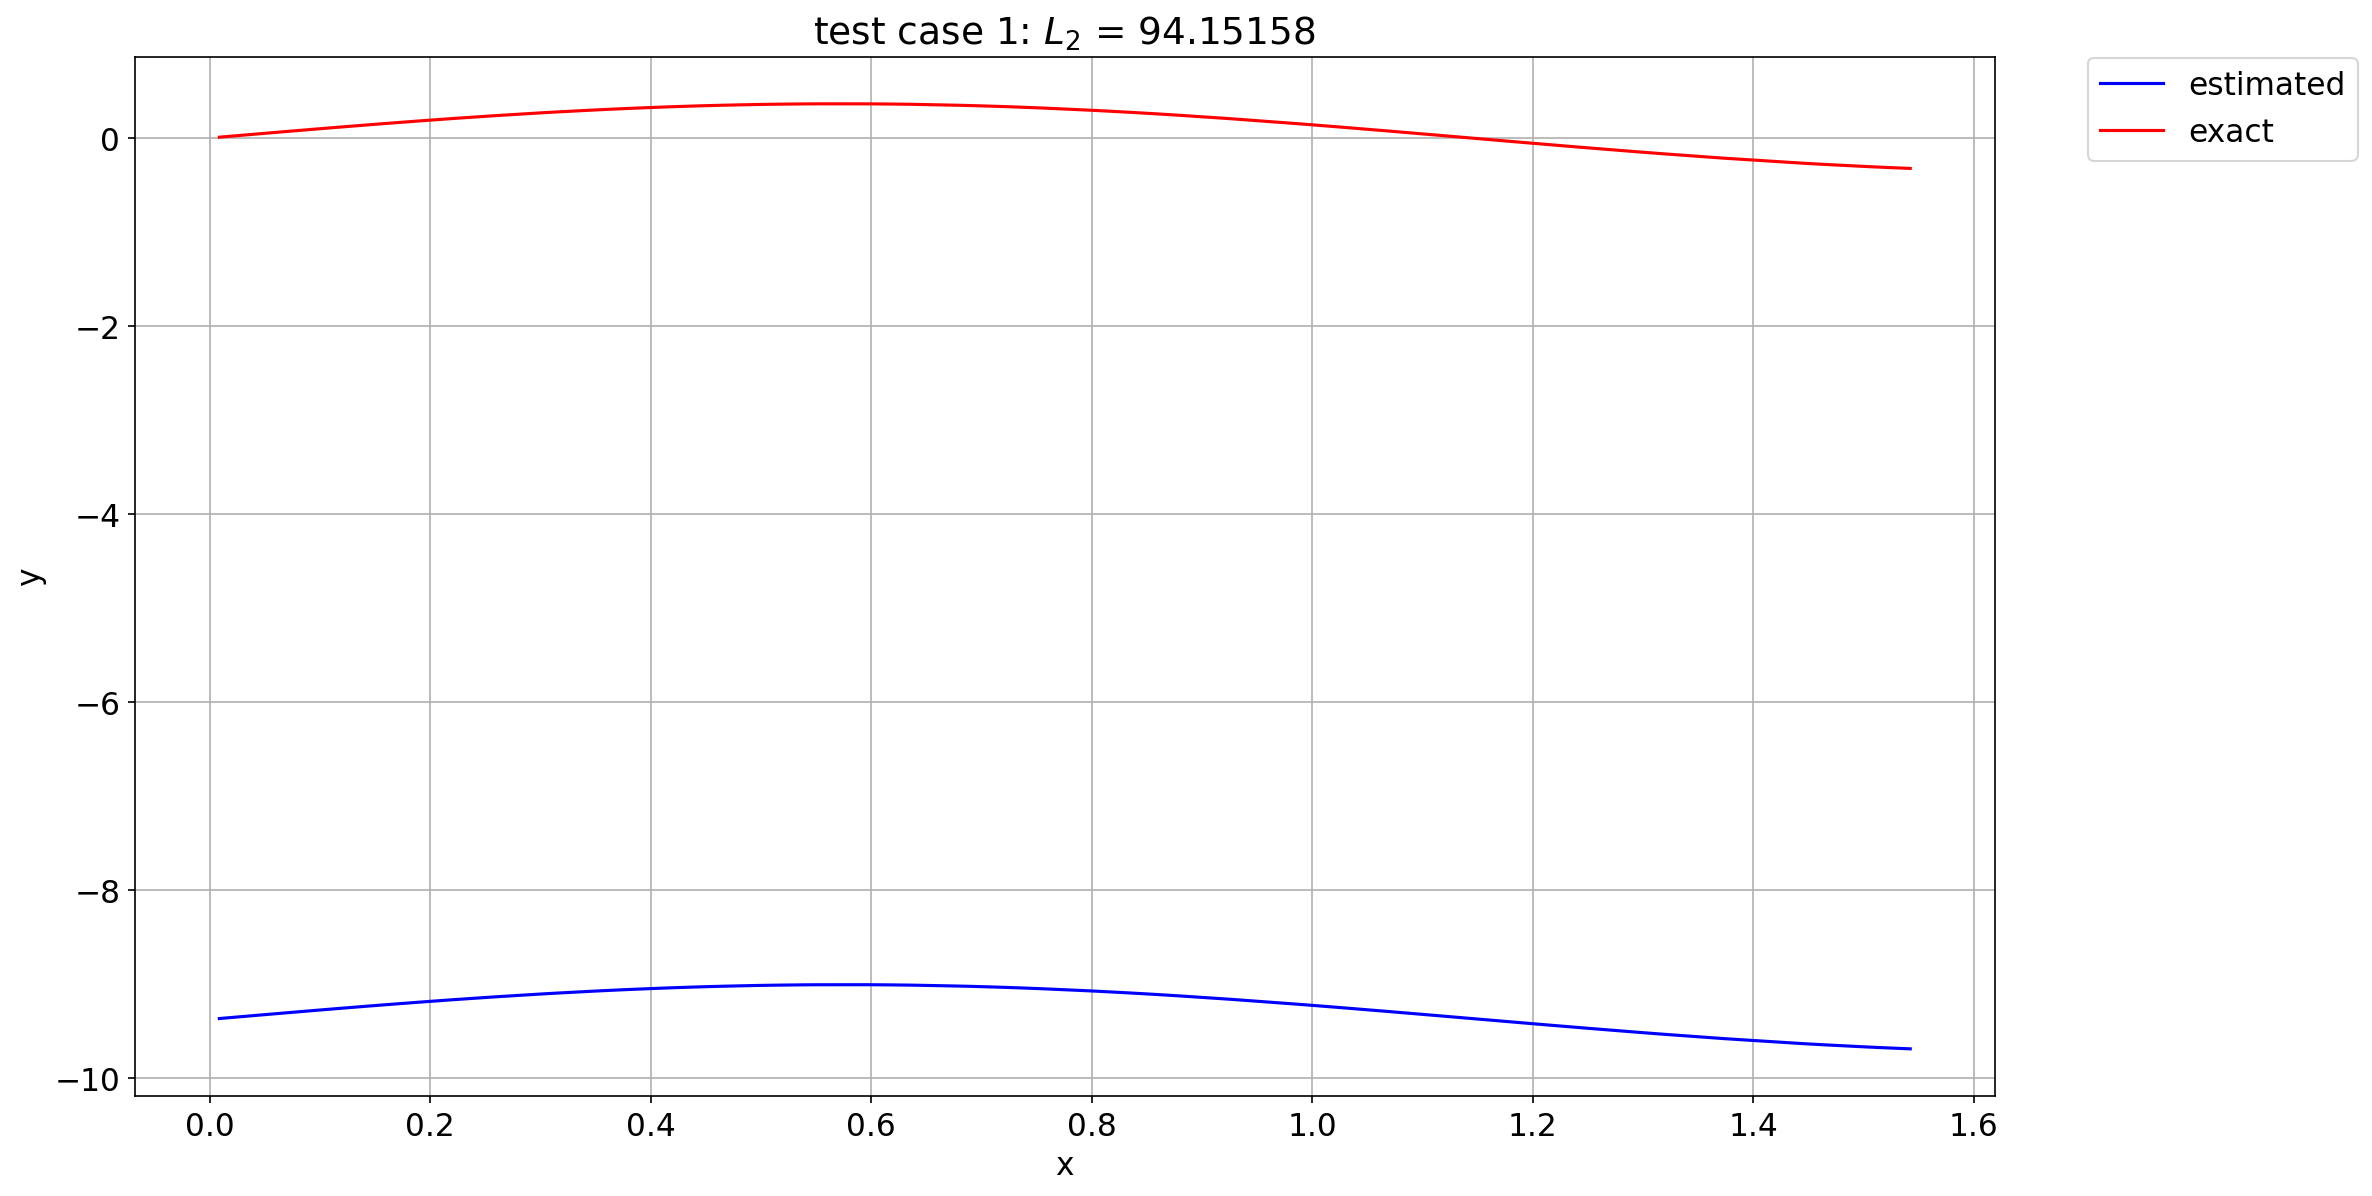
\includegraphics[scale=0.32]{supportingFiles/PI_DON_results/01_originalOutput/test_case_1.png}\hspace{5cm}
    }
\end{frame}

\begin{frame}
    \frametitle{Physics Informed Deep-o-net - results}
    \hbox{\hspace{-1cm}
        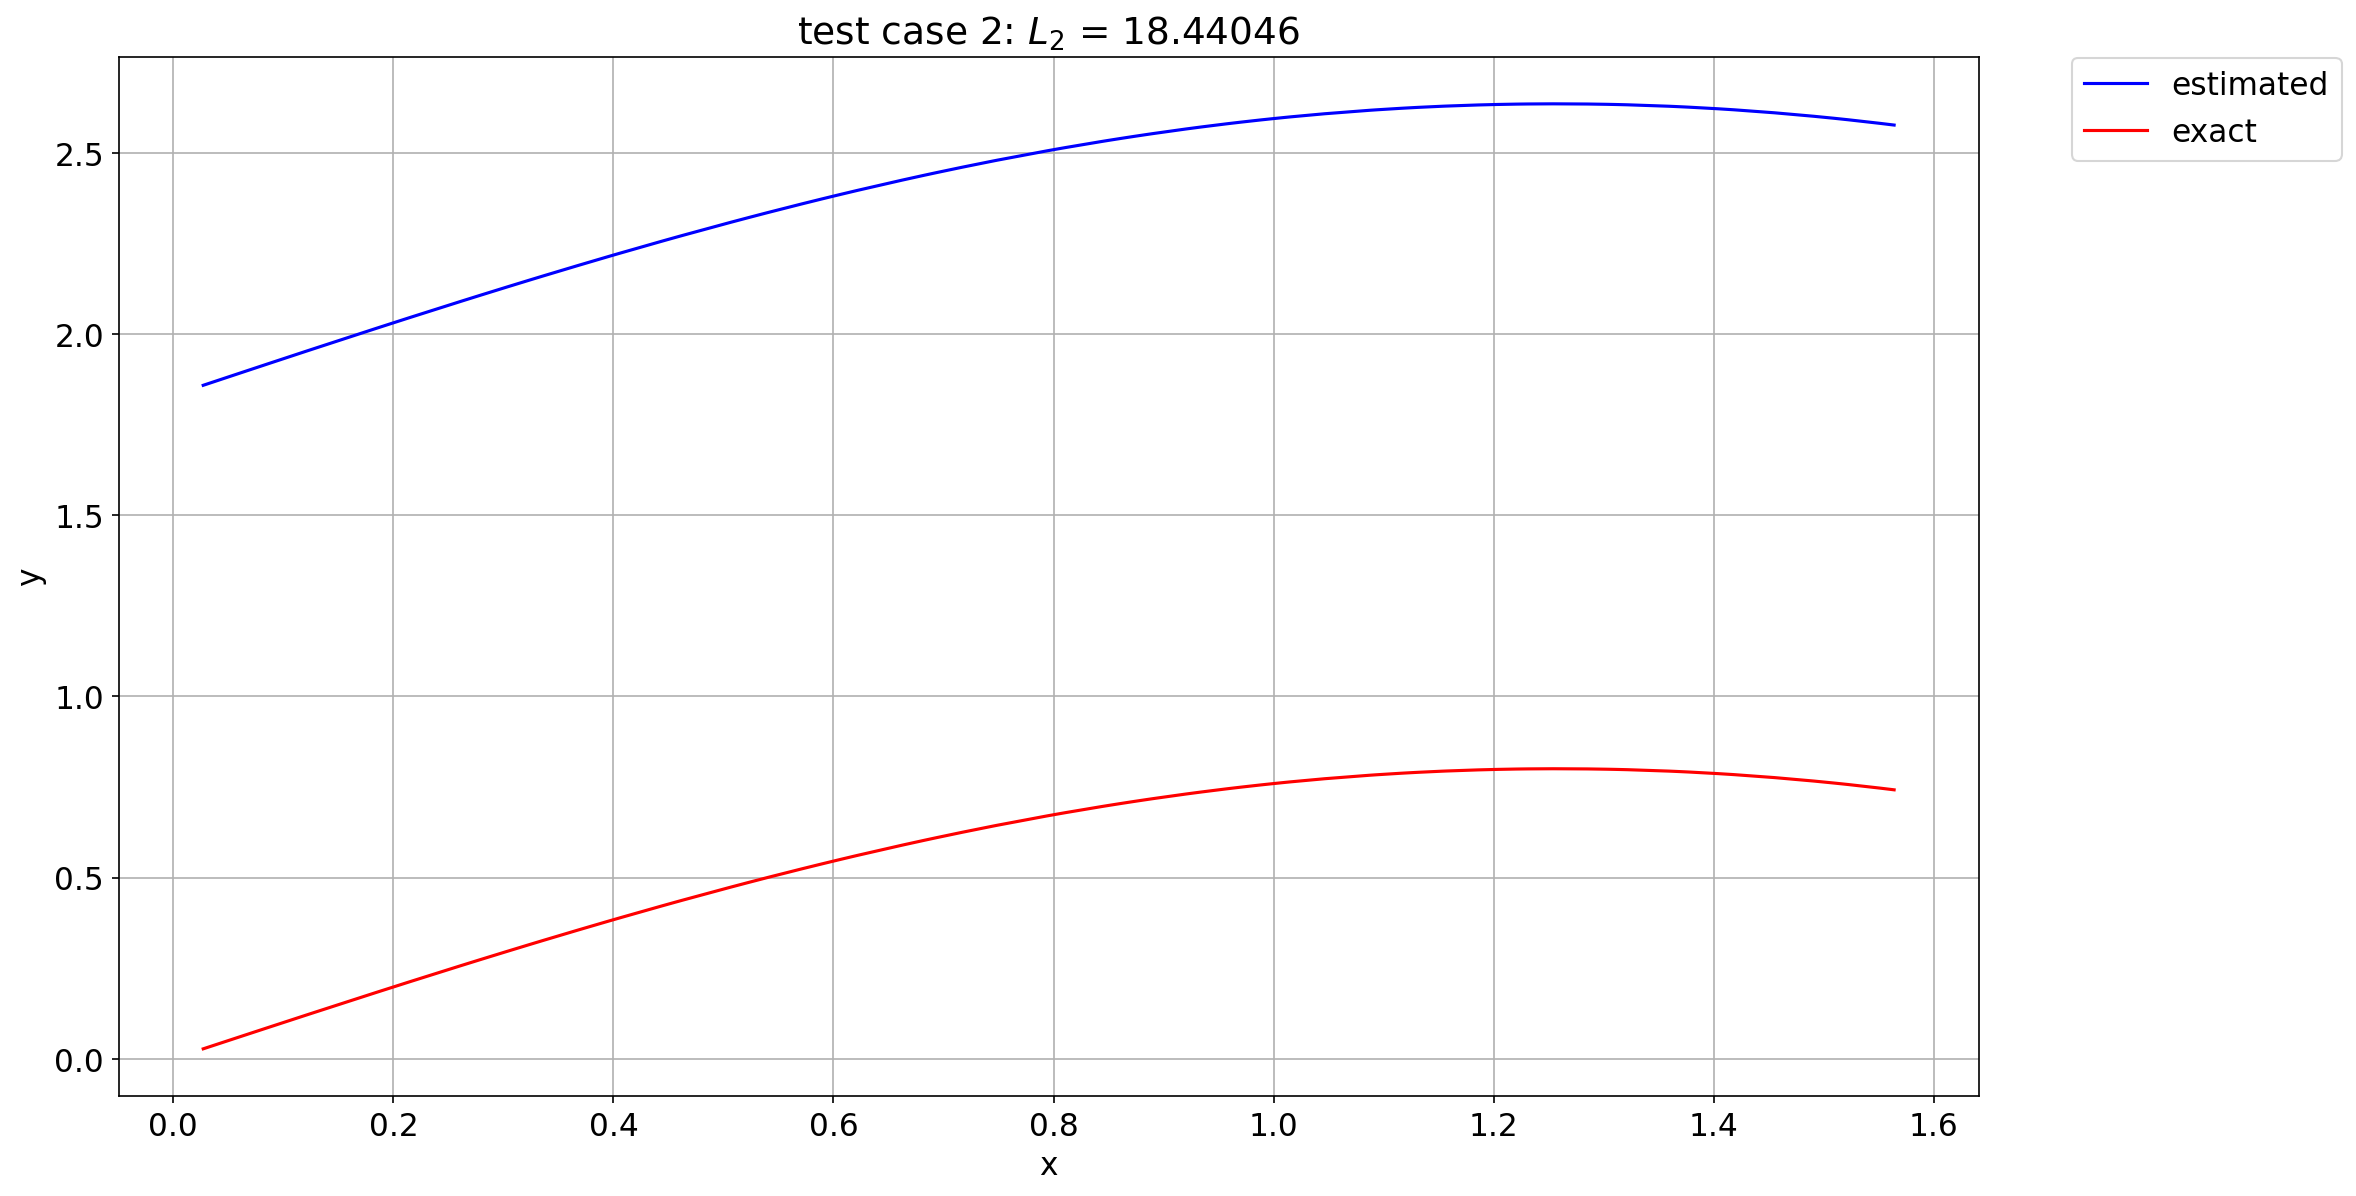
\includegraphics[scale=0.32]{supportingFiles/PI_DON_results/01_originalOutput/test_case_2.png}\hspace{5cm}
    }
\end{frame}

\begin{frame}
    \frametitle{Physics Informed Deep-o-net - results}
    \hbox{\hspace{-1cm}
        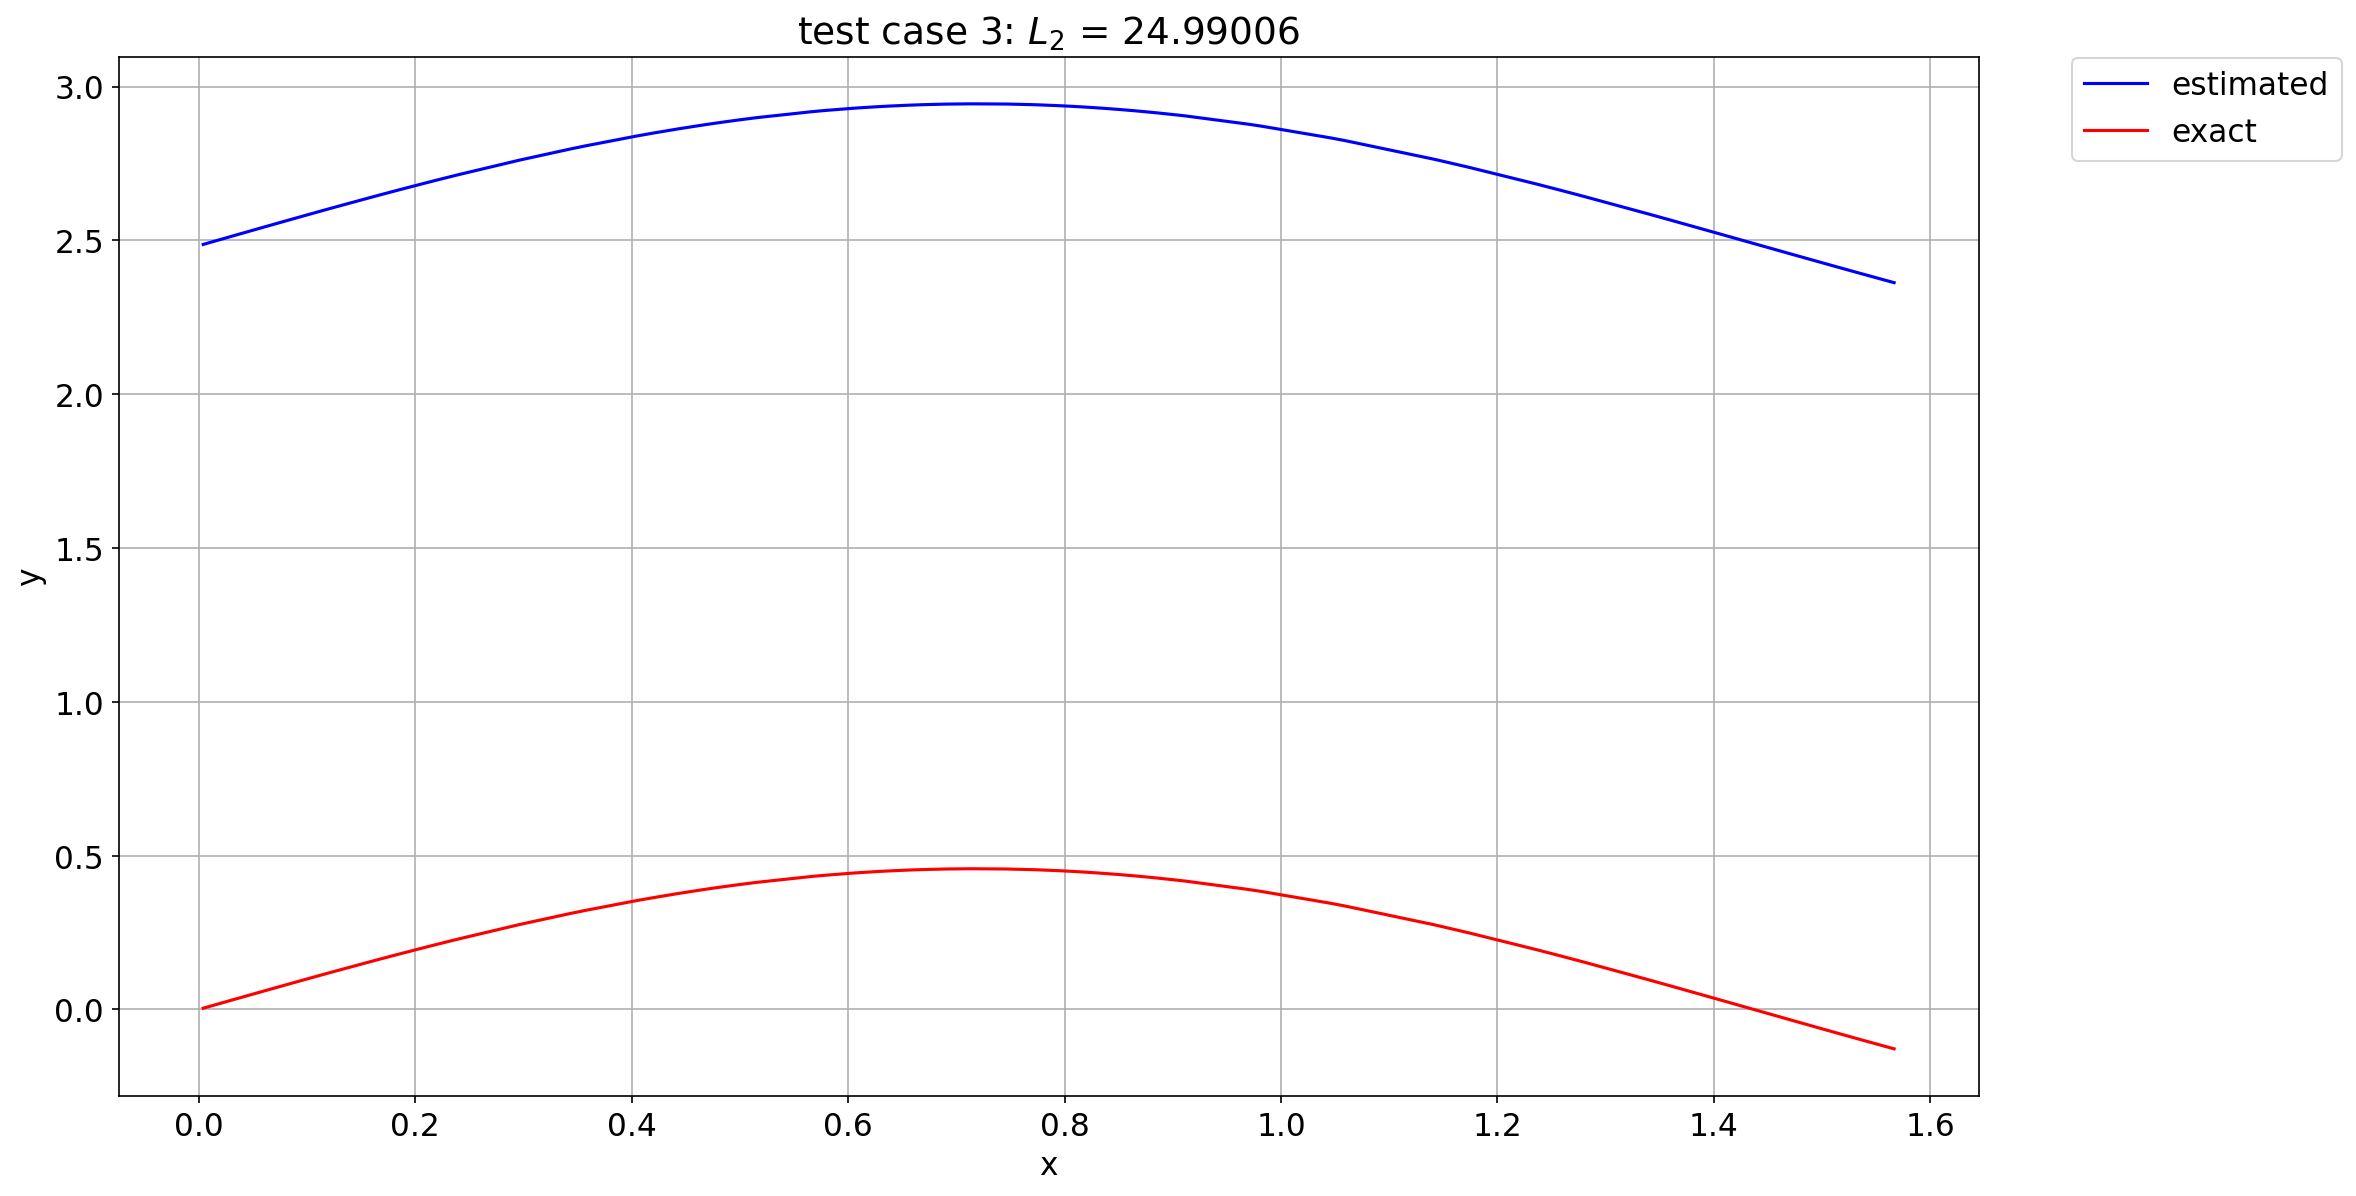
\includegraphics[scale=0.32]{supportingFiles/PI_DON_results/01_originalOutput/test_case_3.png}\hspace{5cm}
    }
\end{frame}

\begin{frame}
    \frametitle{Physics Informed Deep-o-net - results}
    \hbox{\hspace{-1cm}
        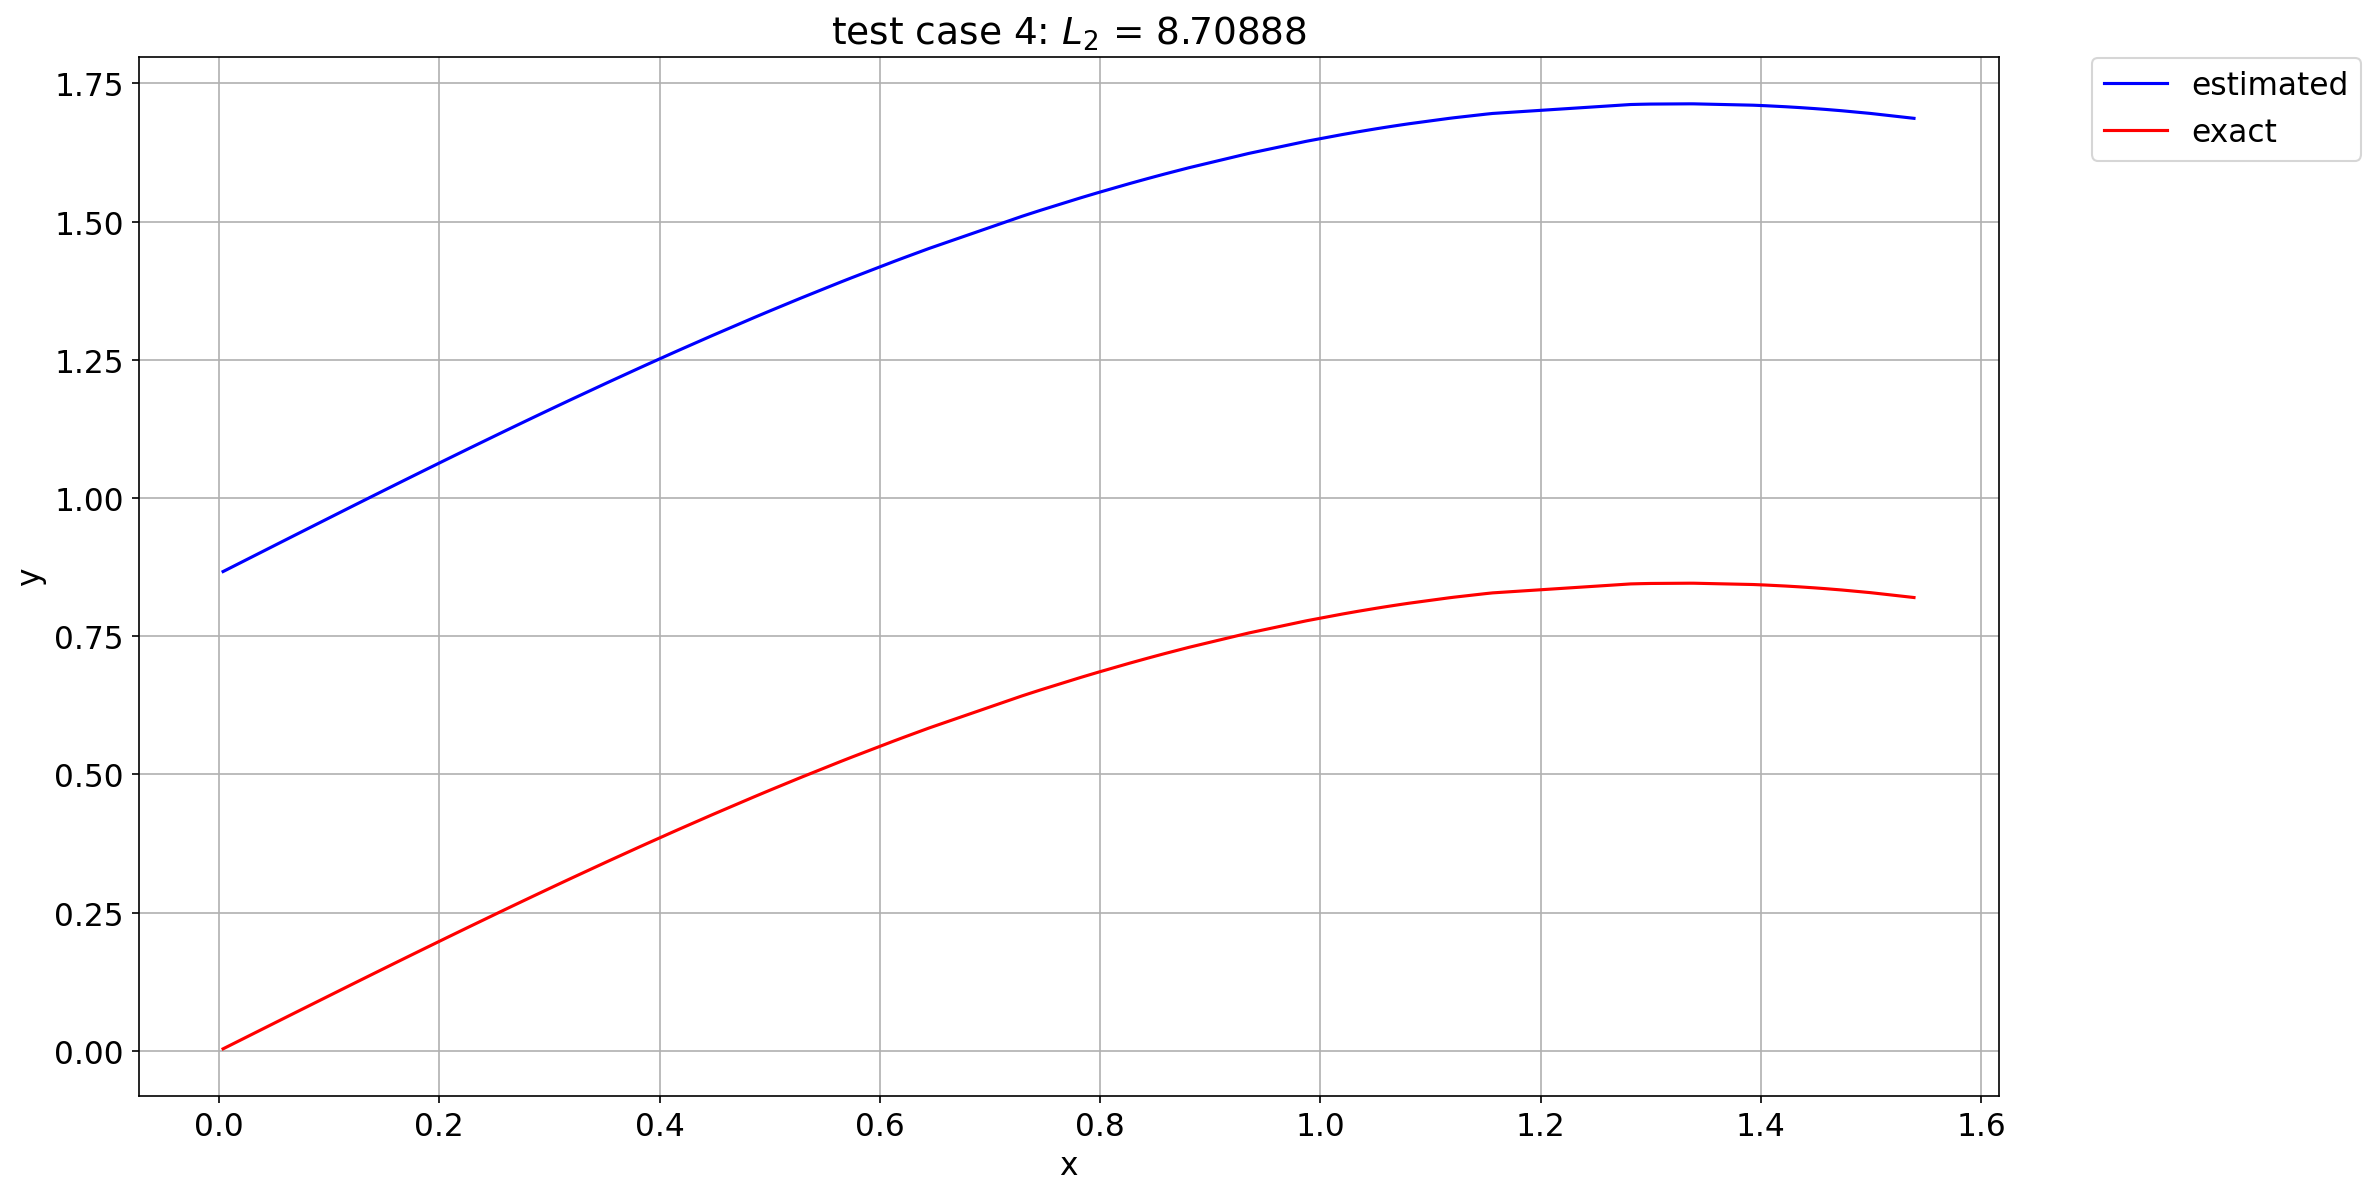
\includegraphics[scale=0.32]{supportingFiles/PI_DON_results/01_originalOutput/test_case_4.png}\hspace{5cm}
    }
\end{frame}

\begin{frame}
    \frametitle{Physics Informed Deep-o-net - results}
    \hbox{\hspace{-1cm}
        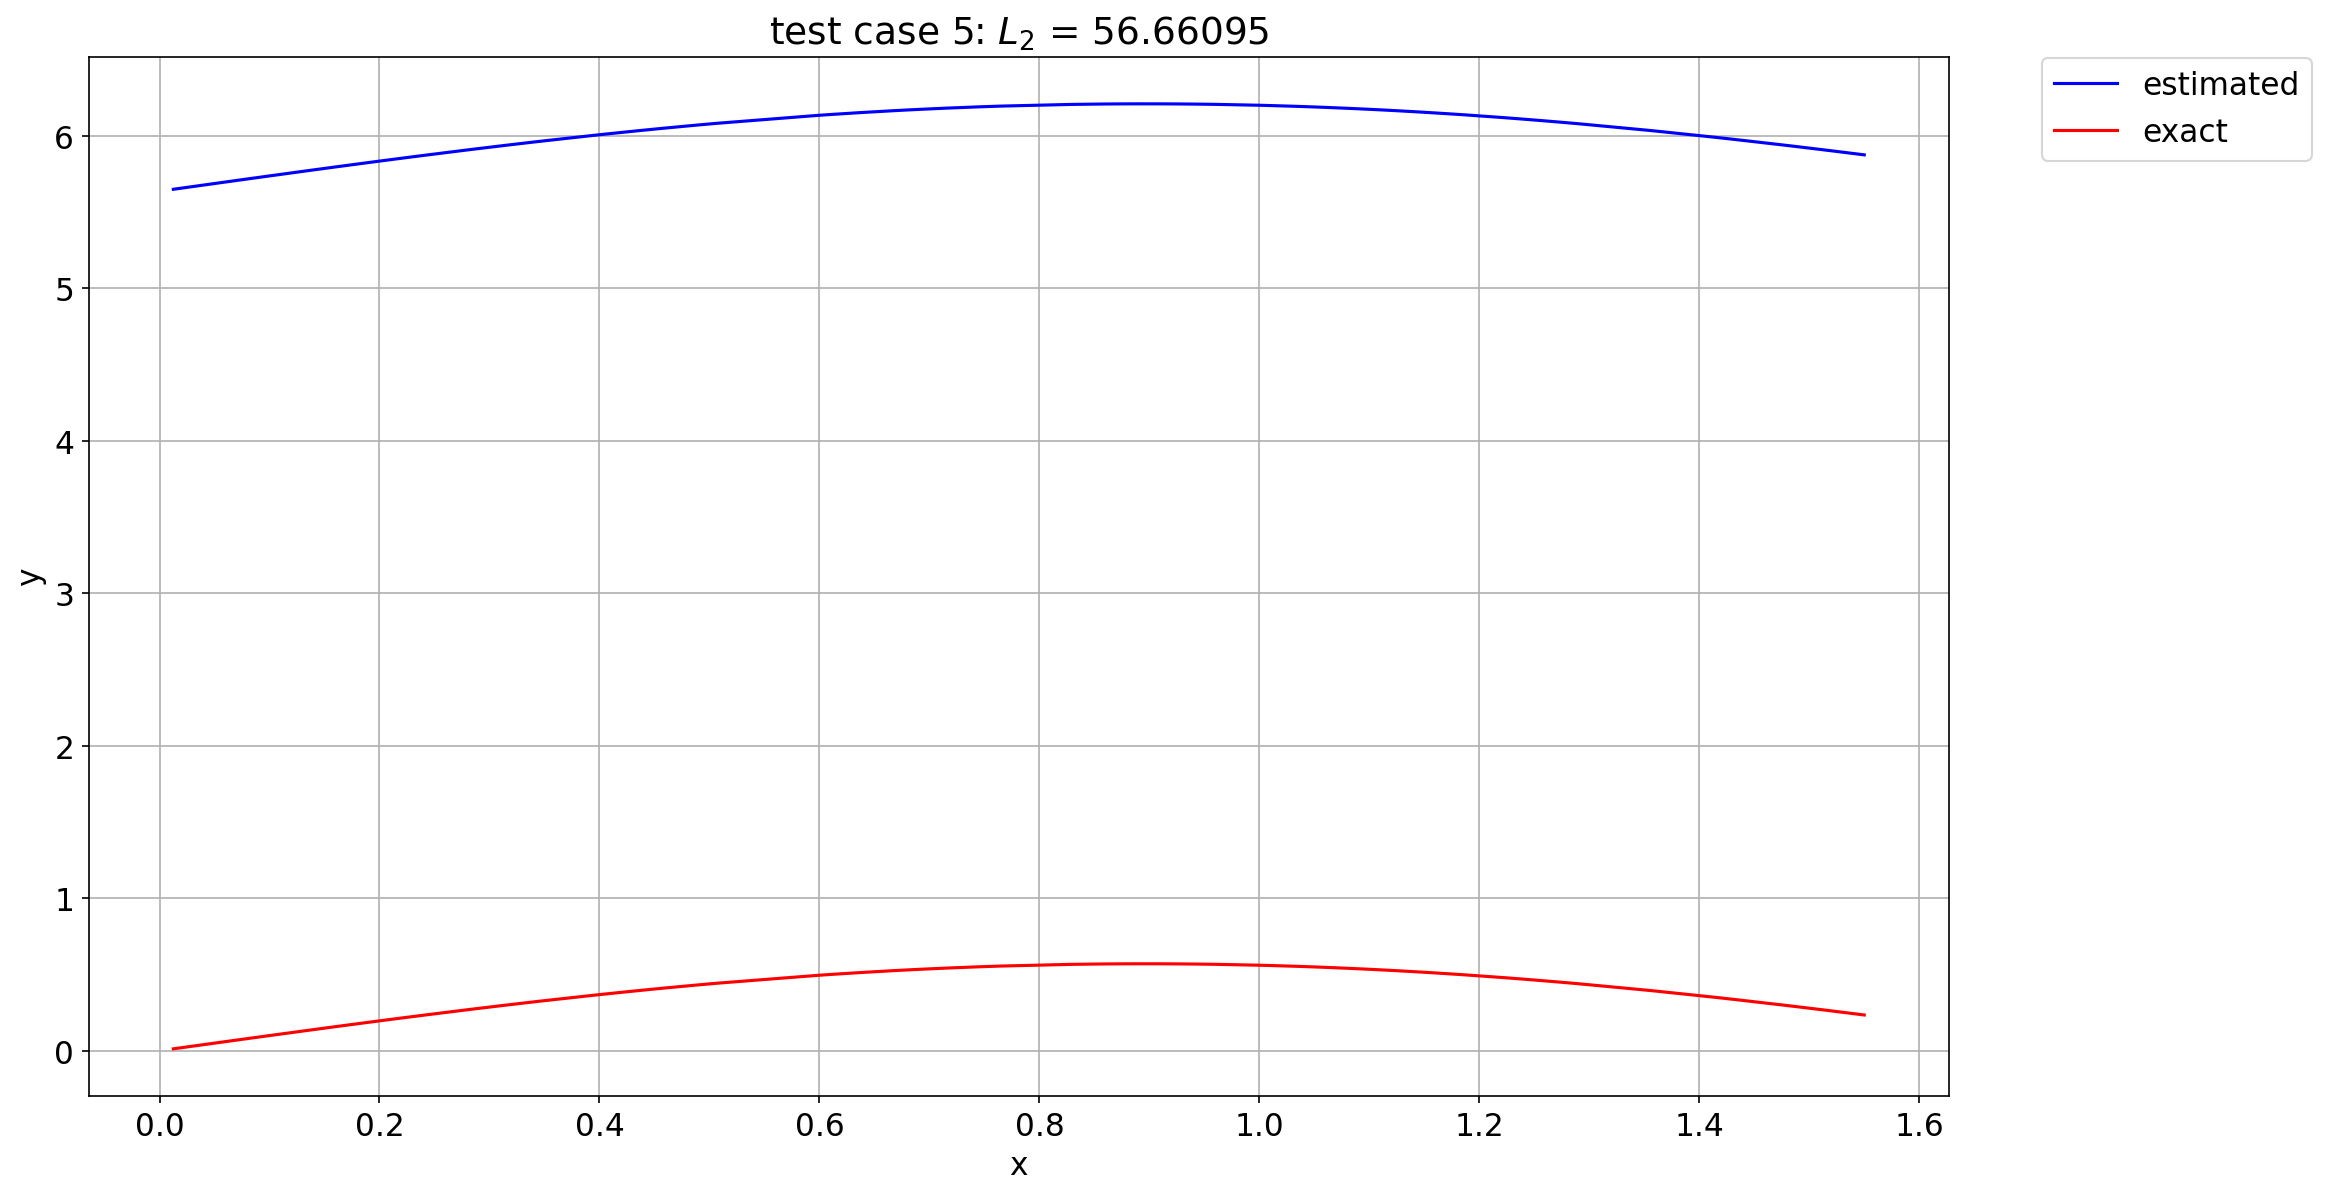
\includegraphics[scale=0.32]{supportingFiles/PI_DON_results/01_originalOutput/test_case_5.png}\hspace{5cm}
    }
\end{frame}

%------------------------------------------------------------------------------
\begin{frame}
    \frametitle{Physics Informed Deep-o-net - Results not mached}
    \onslide<2->{
        Why?
    } \\
    \vspace{0.75cm}

    \onslide<3->{
        Approximating, \(\hat{G}: \cos(\omega t) \to x\)
    } \\

    \vspace{0.75cm}
    \onslide<4->{
        With constraint, \(\frac{d x}{dt} = \cos(\omega t)\)
    } \\

    \vspace{0.75cm}
    \onslide<5->{
        What operator we try to approximate?
    }
    \onslide<6->{
        \(\frac{d}{dt}\left(.\right)\) ?
    }

    \vspace{0.75cm}
    \onslide<7->{
        \textcolor{blue}{Integral Operator}
    }
    \vspace{0.75cm}

    \onslide<8->{
        \(x = \int cos(\omega t)\)
    }
    \onslide<9->{
        \textcolor{red}{
            \(\bm{+ \; \; \; C}\)}
    }

\end{frame}

%------------------------------------------------------------------------------
\begin{frame}
    \frametitle{Physics Informed Deep-o-net - integral constant}

    \begin{figure}
       \center
        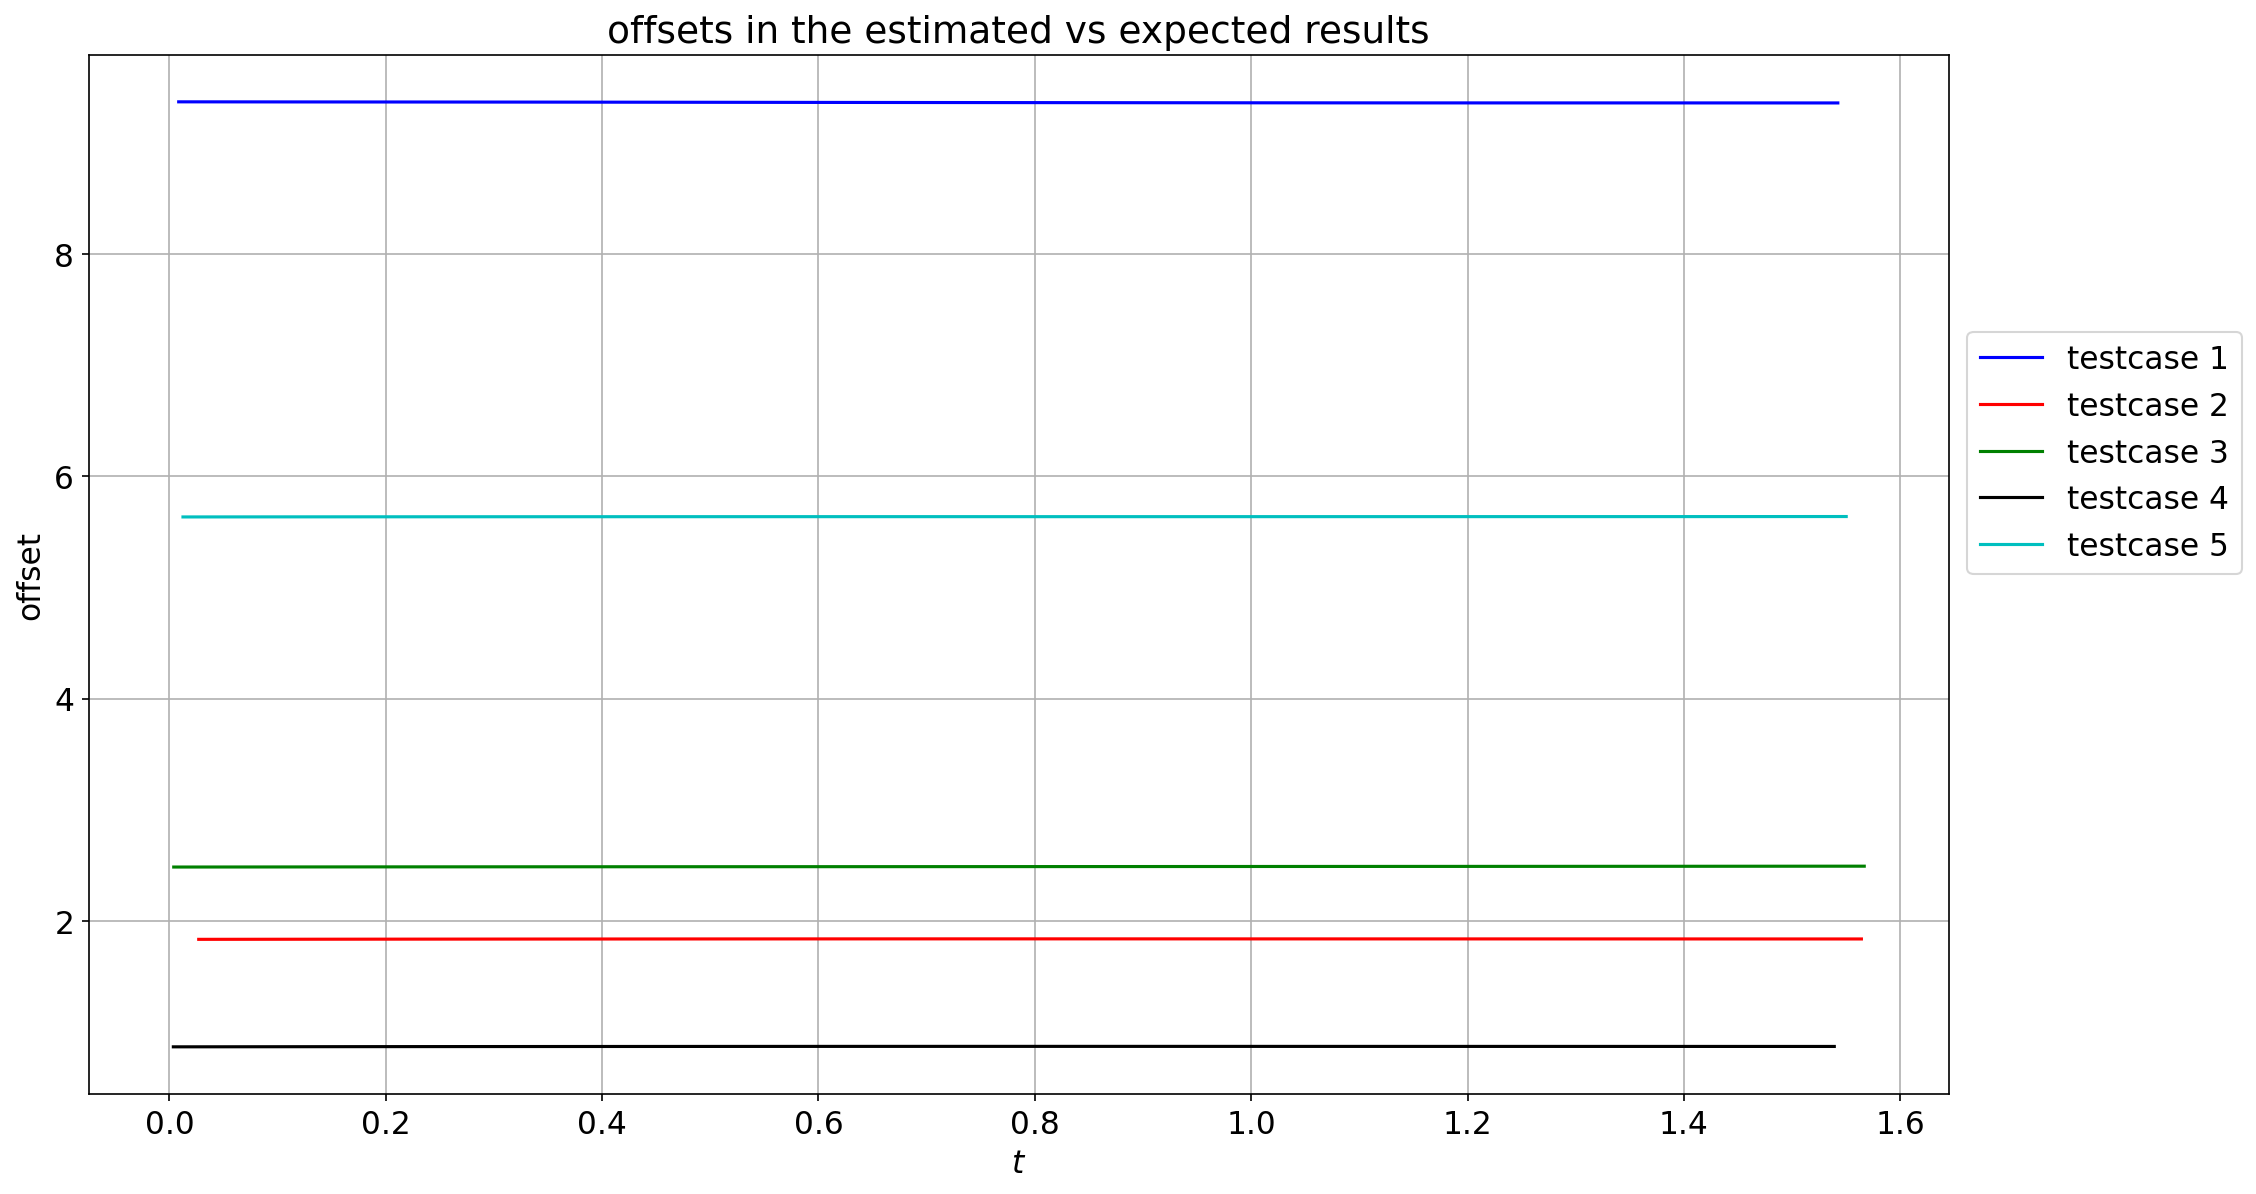
\includegraphics[scale=0.31]{supportingFiles/PI_DON_results/02_correctedOutput/offsets.png}
    \end{figure}

\end{frame}

%------------------------------------------------------------------------------
\begin{frame}
    \frametitle{Physics Informed Deep-o-net - corrected results}
    \hbox{\hspace{-1cm}
        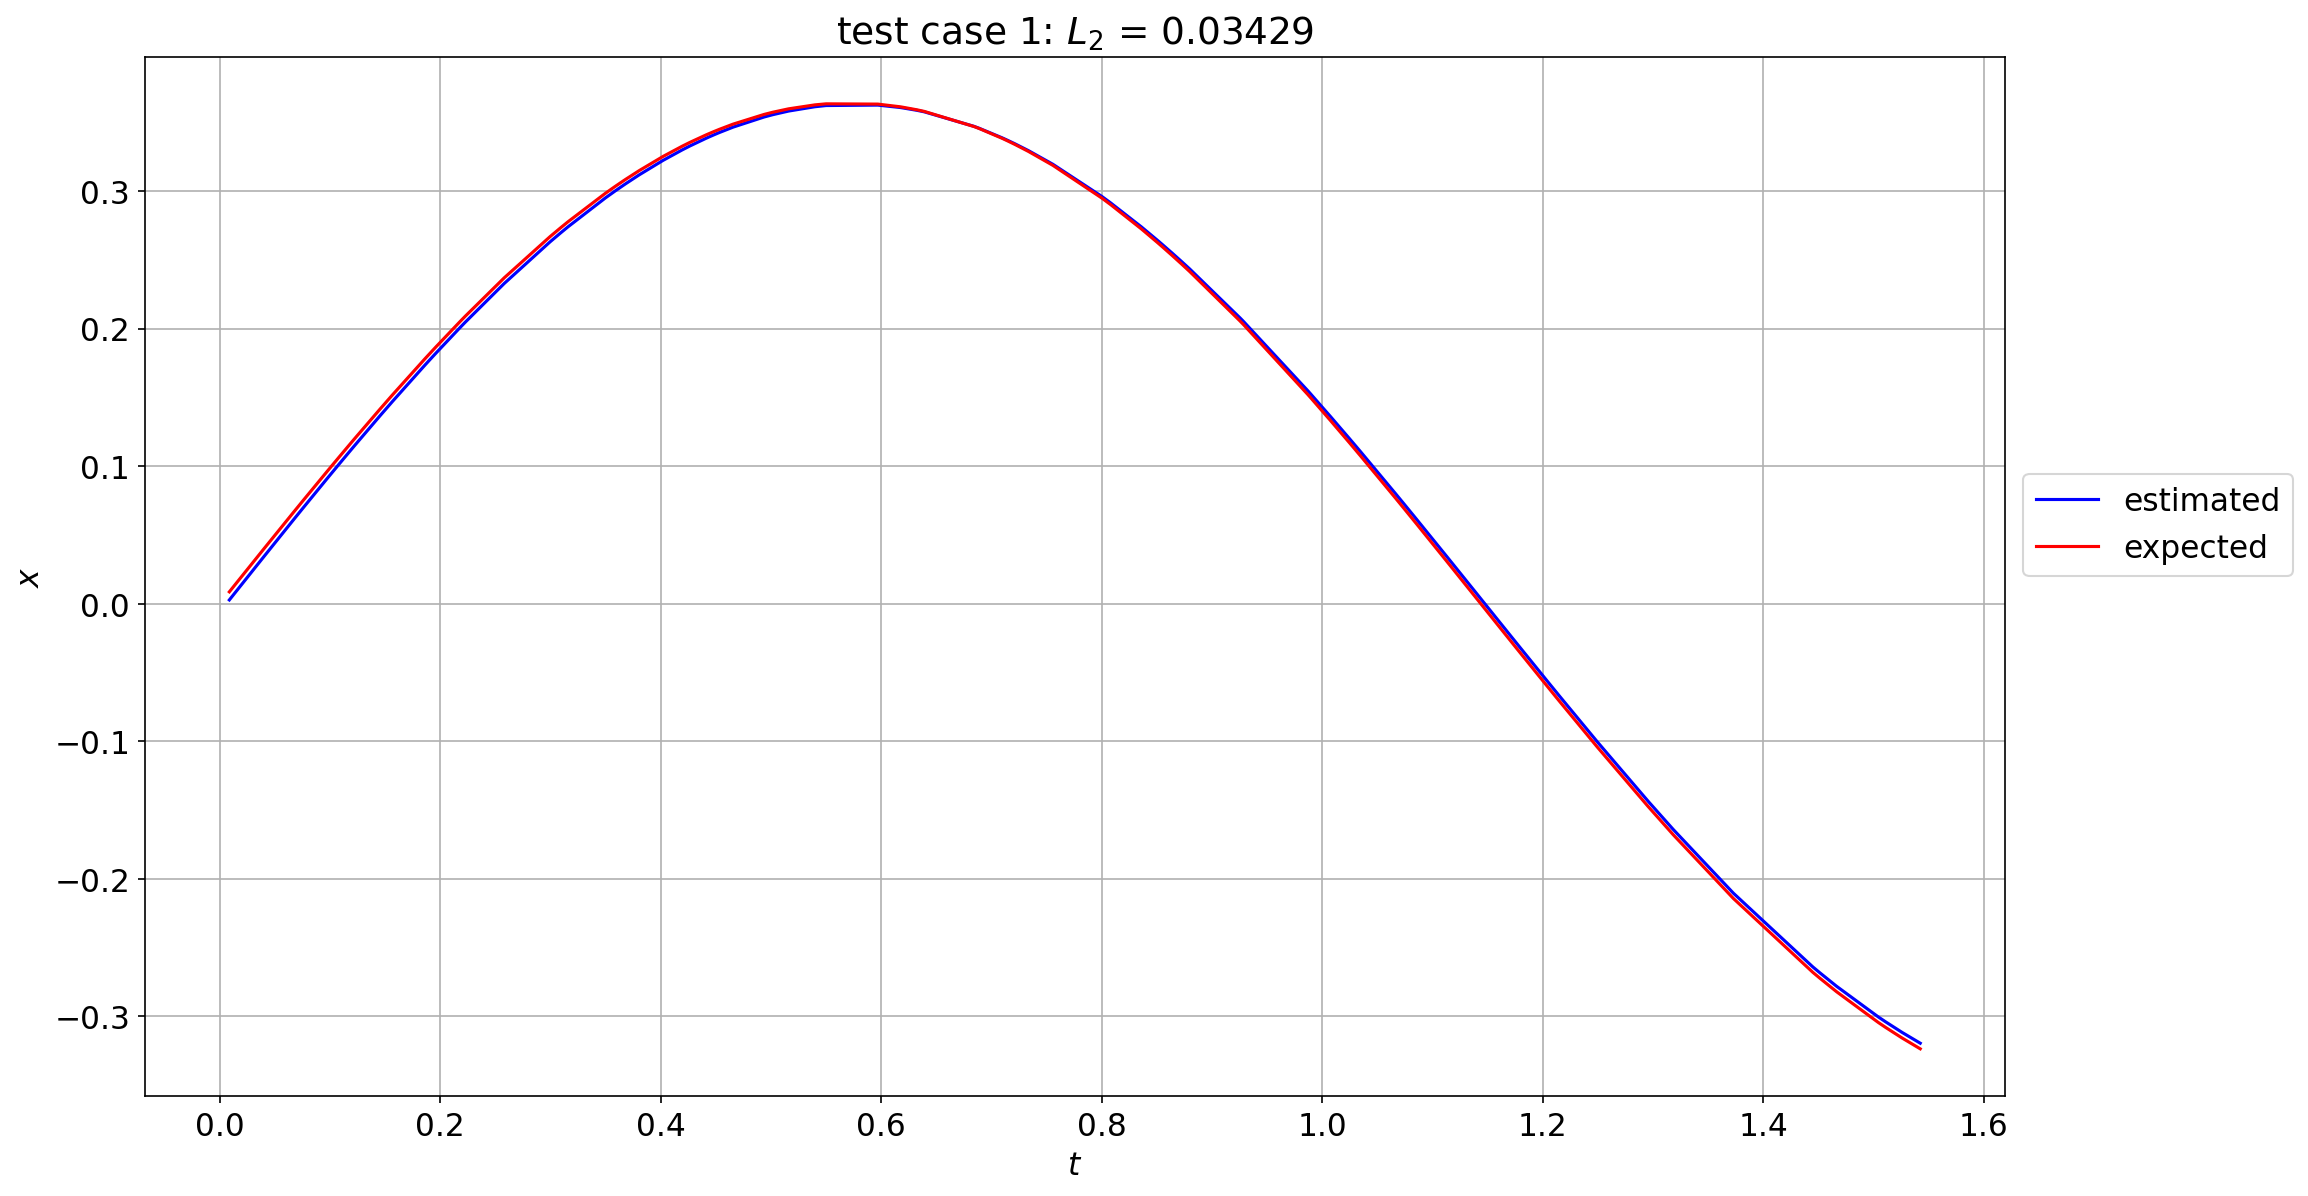
\includegraphics[scale=0.32]{supportingFiles/PI_DON_results/02_correctedOutput/test_case_1_corrected.png}\hspace{5cm}
    }
\end{frame}

\begin{frame}
    \frametitle{Physics Informed Deep-o-net - corrected results}
    \hbox{\hspace{-1cm}
        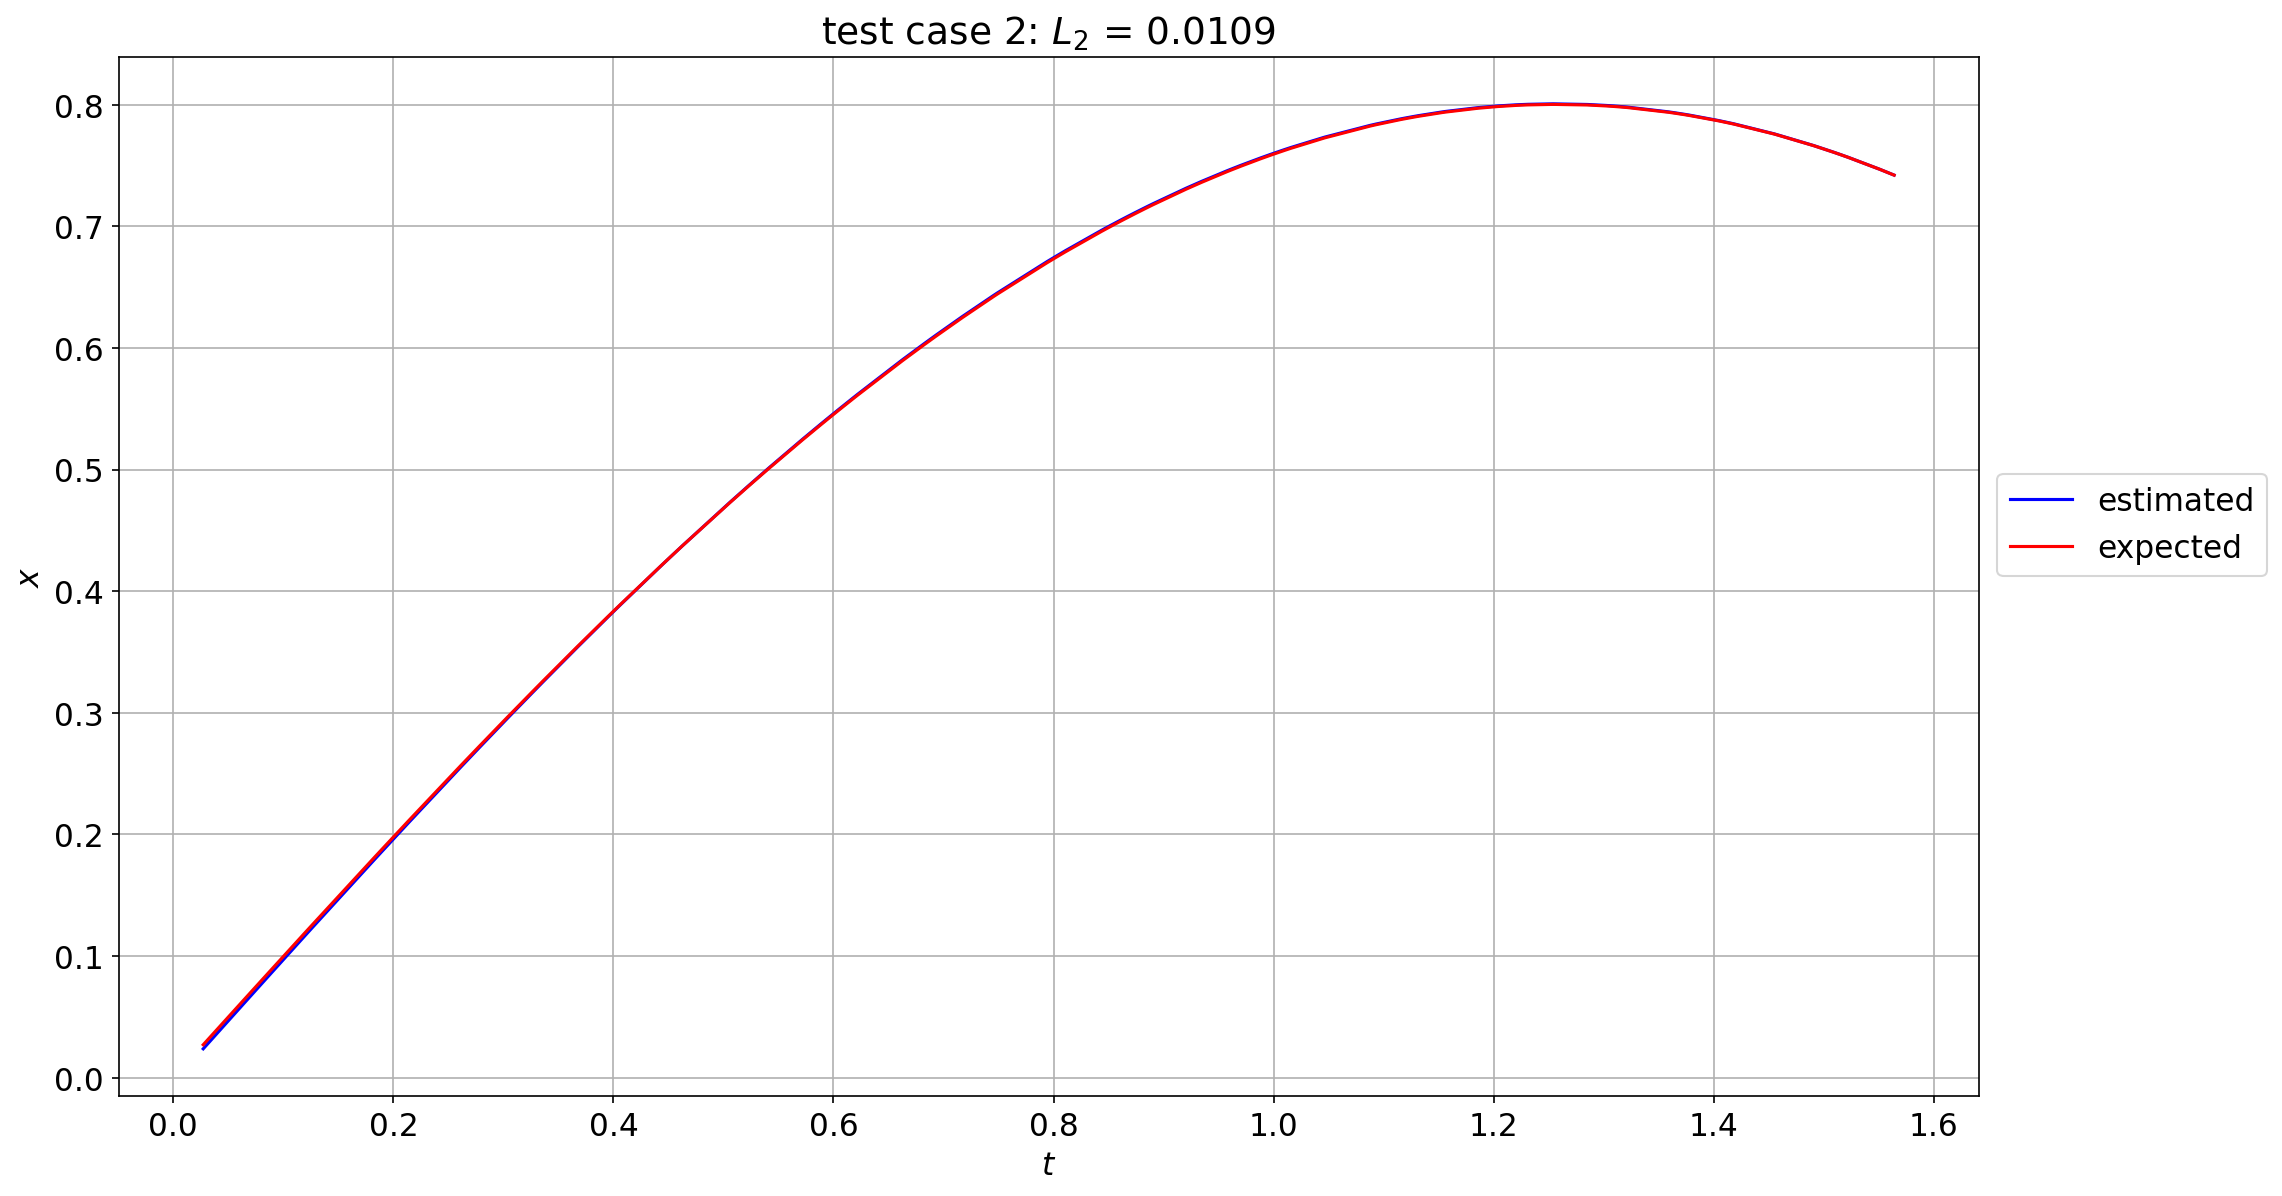
\includegraphics[scale=0.32]{supportingFiles/PI_DON_results/02_correctedOutput/test_case_2_corrected.png}\hspace{5cm}
    }
\end{frame}

\begin{frame}
    \frametitle{Physics Informed Deep-o-net - corrected results}
    \hbox{\hspace{-1cm}
        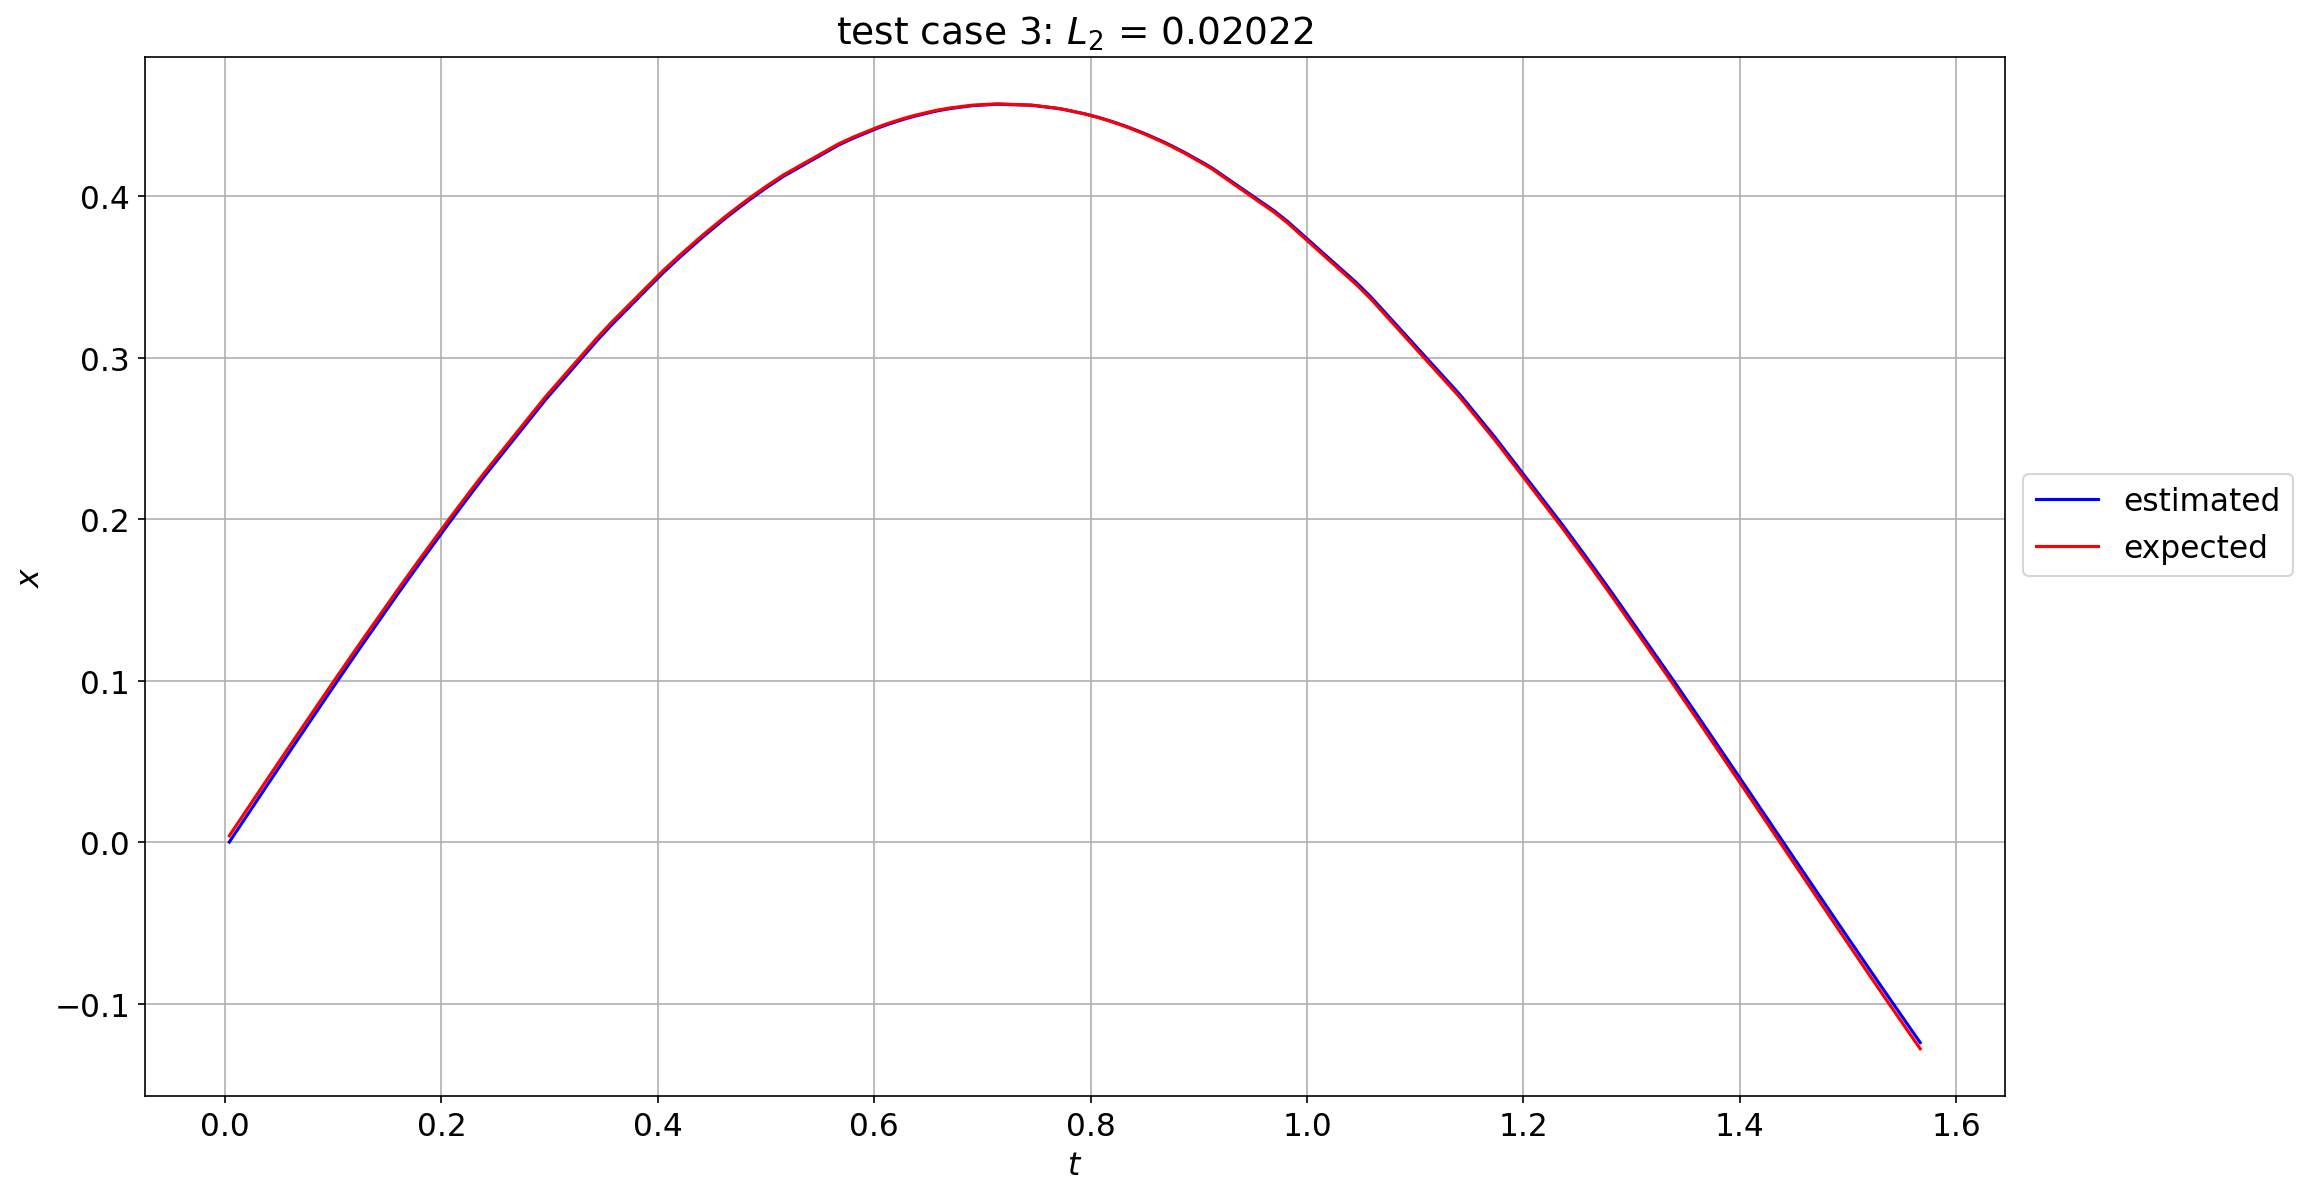
\includegraphics[scale=0.32]{supportingFiles/PI_DON_results/02_correctedOutput/test_case_3_corrected.png}\hspace{5cm}
    }
\end{frame}

\begin{frame}
    \frametitle{Physics Informed Deep-o-net - corrected results}
    \hbox{\hspace{-1cm}
        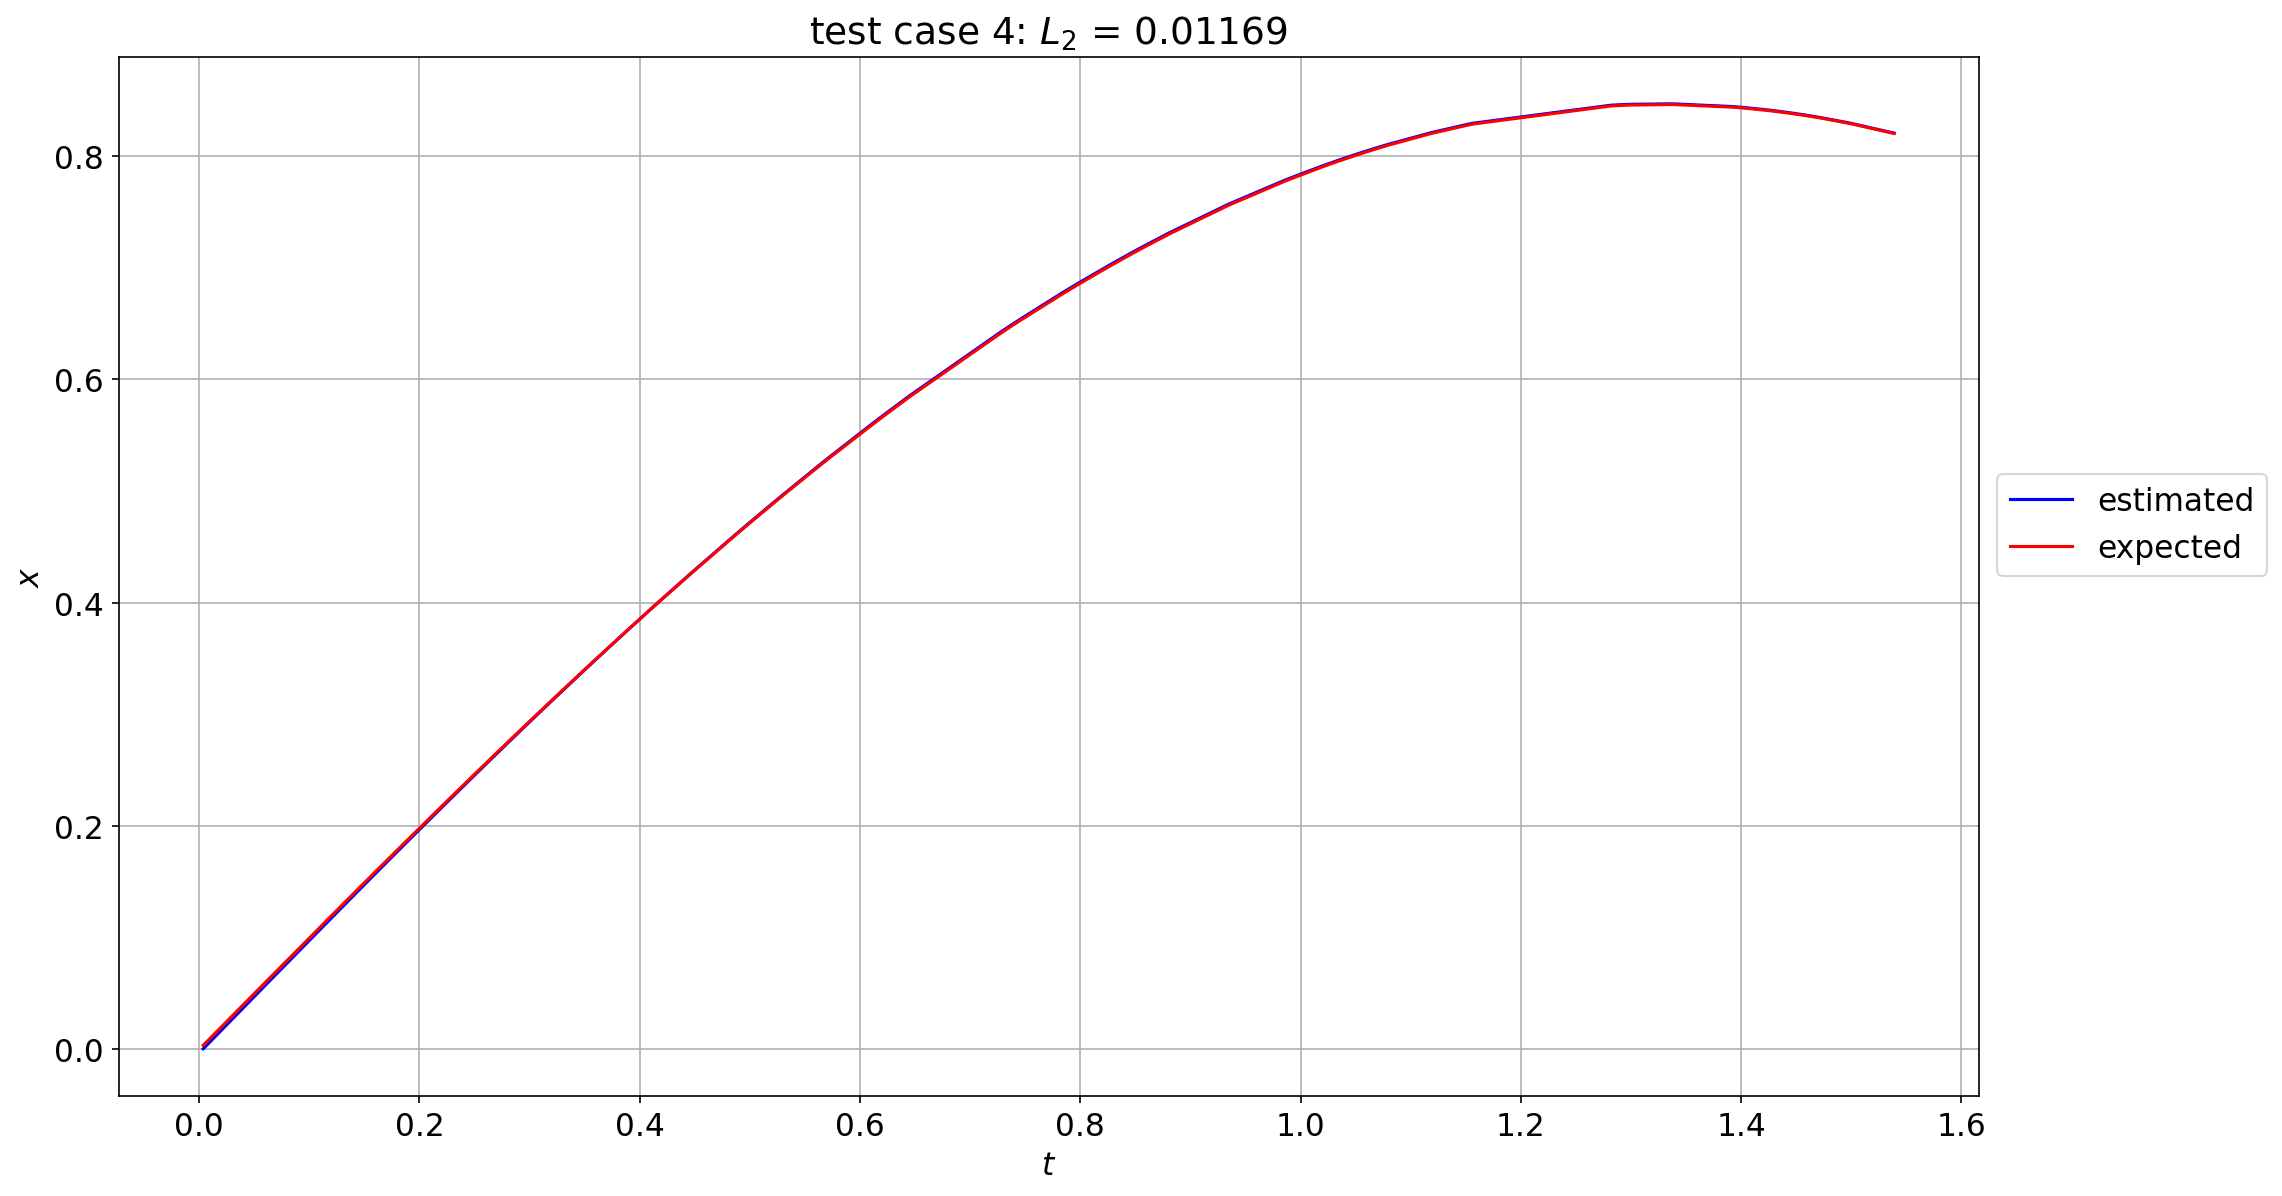
\includegraphics[scale=0.32]{supportingFiles/PI_DON_results/02_correctedOutput/test_case_4_corrected.png}\hspace{5cm}
    }
\end{frame}

\begin{frame}
    \frametitle{Physics Informed Deep-o-net - corrected results}
    \hbox{\hspace{-1cm}
        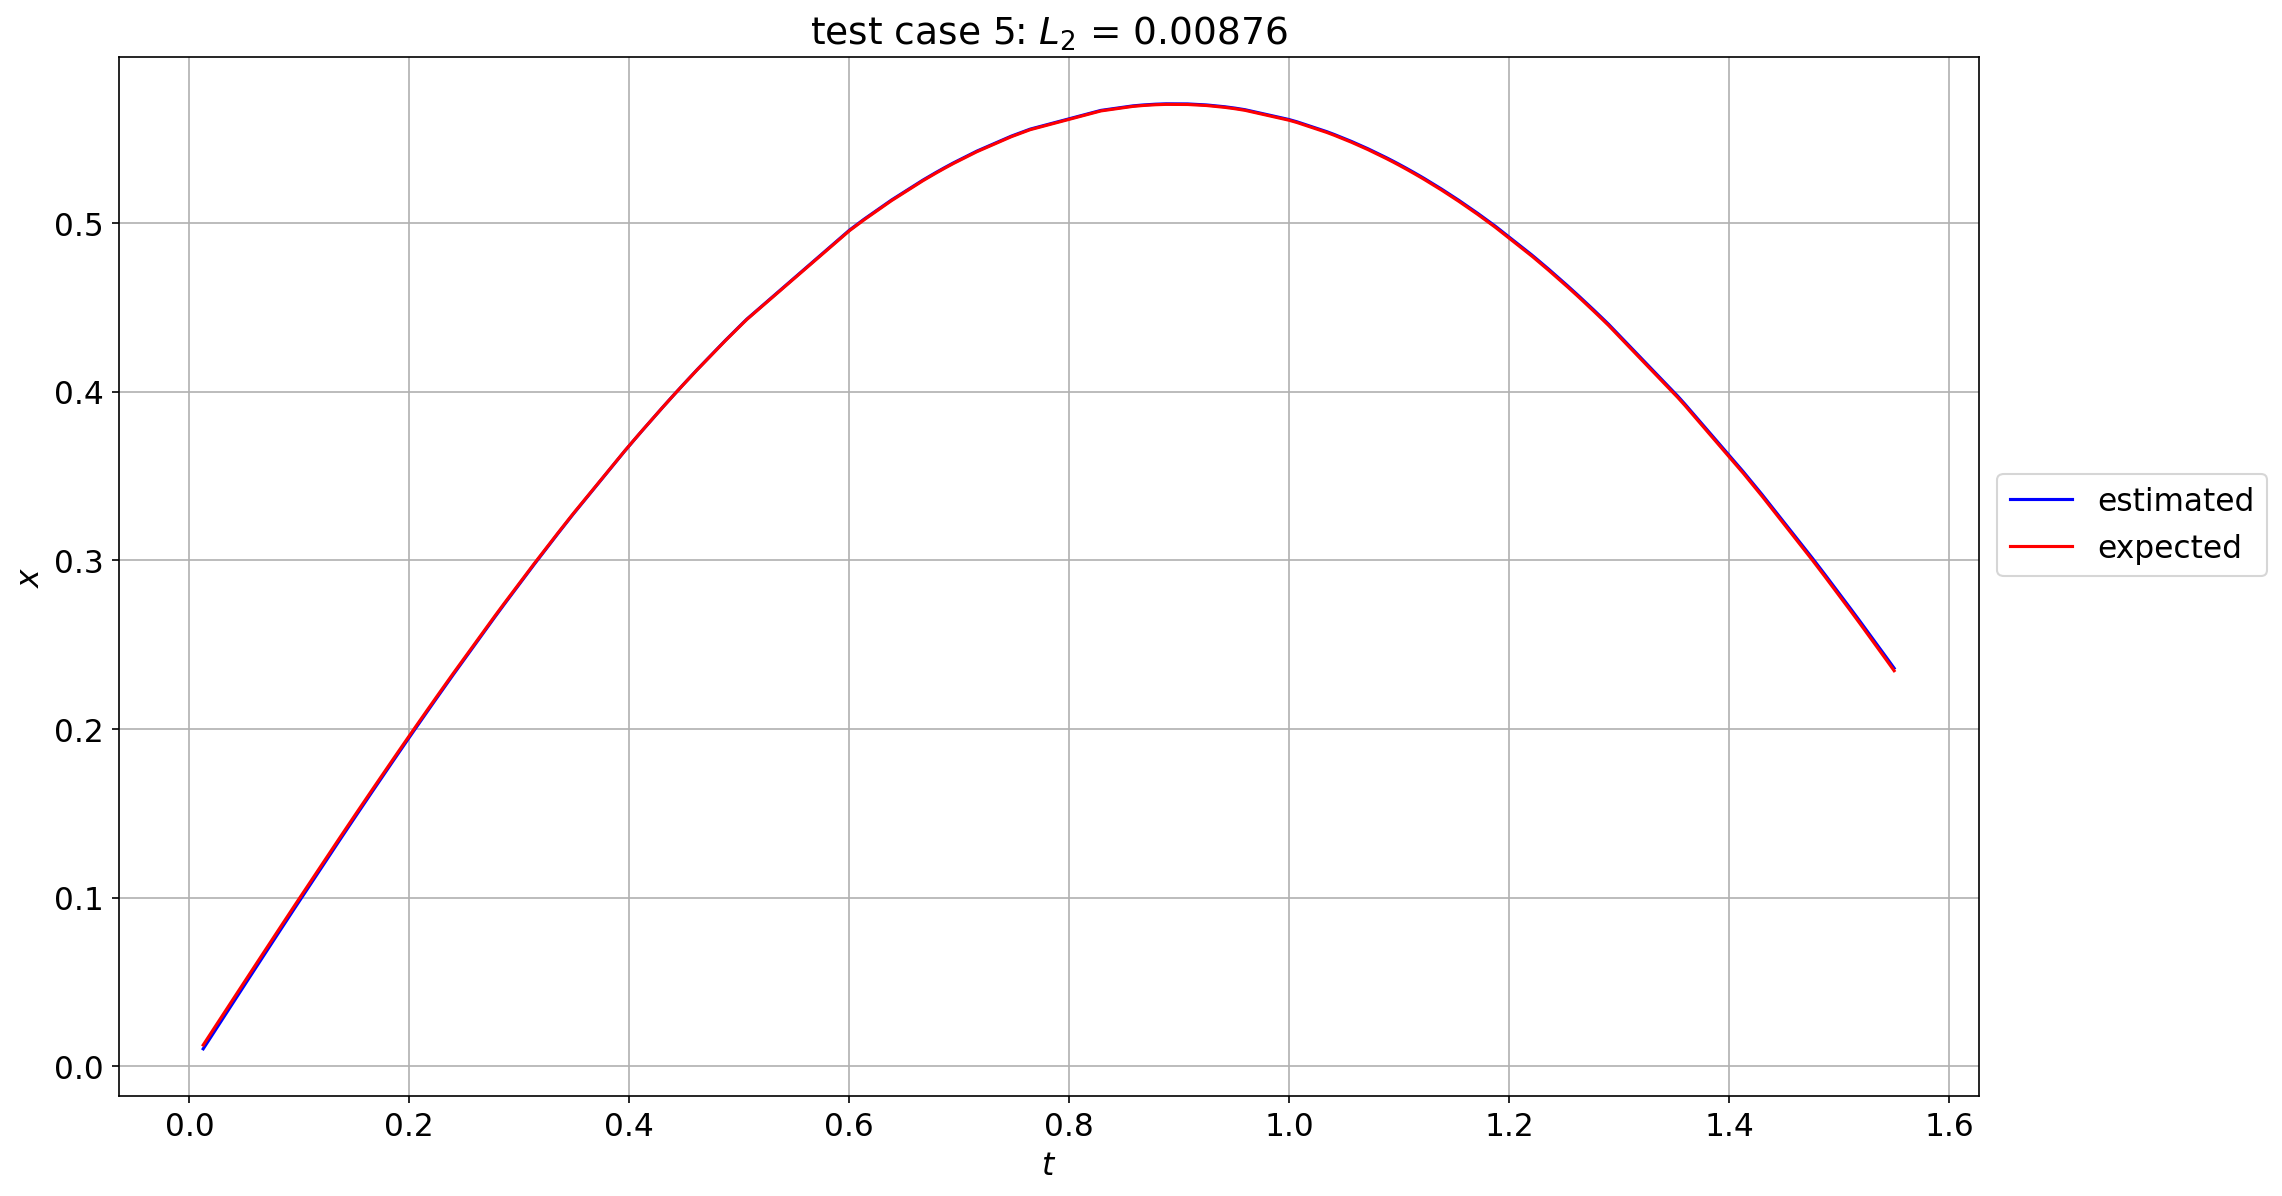
\includegraphics[scale=0.32]{supportingFiles/PI_DON_results/02_correctedOutput/test_case_5_corrected.png}\hspace{5cm}
    }
\end{frame}

%------------------------------------------------------------------------------

\begin{frame}
    \frametitle{Source code}

    Available on github \\

    \vspace{1cm}

    \href{https://github.com}{\textcolor{blue}{https://github.com}}

\end{frame}
